%!TEX root = ComputerScienceOne.tex

%%Chapter: Searching & Sorting

Searching and sorting are two fundamental operations when dealing
with collections of data.  Both operations are not only important in
and of themselves, but they also form the basis of many algorithms
and other more complex operations.  These operations are so essential 
that a wide variety
of algorithms and techniques have been developed to solve them, each
with their own advantages and disadvantages.  This variety provides
a good framework from which to study the relative efficiency and complexity
of algorithms through algorithm analysis.

\section{Searching}
\index{searching}

Searching is a very basic operation.  Given a collection of data, we
wish to find a particular element or elements that match a certain 
criteria.  More formally, we have the following.

\begin{problem}[Searching]
\label{problem:searching}
~\\
\textbf{Given:} a collection of elements, $A =\{a_1, a_2, \ldots, a_n\}$ 
and a \emph{key} element $e_k$\\
\textbf{Output:} The element $a_i$ in $A$ such that $a_i = e_k$
\end{problem}

The ``equality'' in this problem statement is not explicitly 
specified.  In 
fact, this is a very general, abstract statement of the basic search 
problem.  We didn't specify that the ``collection'' was an array, a list, 
a set, or any other particular data structure.  Nor did we specify what
type of elements were in the collection.  They could be numbers, they
could be strings, they could be objects.  

There are many variations of this general search problem that we could
consider.  For example, we could generalize it to find the ``first''
or ``last'' such element if our collection is ordered.  We could find
\emph{all} elements that match our criteria.  Some basic operations that 
we've already considered such as finding the minimum or maximum
(\emph{extremal} elements), or median element are also variations on this search 
problem.

When designing a solution to any of these variations additional 
considerations must be made.  We may wish our search to be index-based 
(that is, output the index $i$ rather than the element $a_i$).  We
may need to think about how to handle \emph{unsuccessful} searches 
(return \mintinline{text}{null}?  A special flag value?  Throw an
exception?, etc.).

When implementing a solution in a programming language, we of course
will need to be more specific about the type of collection being
searched and the type of elements in the collection.  However, we
will still want to keep our solution as general as possible.  As we'll 
see, most programming languages facilitate some sort of 
\index{generic programming} \emph{generic}
programming so that we do not need to reimplement the solution for
\emph{each} type of collection or for \emph{each} type of variable.  
Instead, we can write one solution, then \emph{configure} it to allow
for comparisons of any type of variable (numeric, string, object, etc.).

\subsection{Linear Search}
\index{search!linear search}
\index{linear search}

The first solution that we'll look at is the \emph{linear search}
algorithm (also known as sequential search).  This is a basic, 
straightforward solution to the search problem that works by simply
iterating through each element $a_i$, testing for equality, and
outputting the first element that matches the criteria.  The
pseudocode is presented as Algorithm \ref{algo:linearSearch}.

\begin{algorithm}[H]
  \Input{A collection of elements $A = \{a_1, \ldots, a_n\}$ and a key $e_k$}
  \Output{An element $a$ in $A$ such that $a = e_k$ according to some criteria; $\phi$ if no such element exists}
  \ForEach{$a_i \textrm{ in the collection } A$}{
    \If{$a_i = e_k$}{ \label{algo:linearSearch:elemOp}
      output $a_i$ \;
    }
  }
  output $\phi$ \;
\caption{Linear Search}
\label{algo:linearSearch}
\end{algorithm}

To illustrate, consider the following example searches.  Suppose we wish
to search the 0-indexed array of integers in Figure \ref{figure:arrayForSearching}.

%\documentclass[12pt]{scrbook}
%
%\usepackage{tikz}
%\usepackage{minted}
%\usetikzlibrary{decorations.pathreplacing,arrows}
%
%\usepackage{fullpage}
%\usepackage{subfigure}
%\begin{document}
%
%
%Lorem Ipsum is simply dummy text of the printing and typesetting industry. Lorem Ipsum has been the industry's standard dummy text ever since the 1500s, when an unknown printer took a galley of type and scrambled it to make a type specimen book. It has survived not only five centuries, but also the leap into electronic typesetting, remaining essentially unchanged. It was popularised in the 1960s with the release of Letraset sheets containing Lorem Ipsum passages, and more recently with desktop publishing software like Aldus PageMaker including versions of Lorem Ipsum.

\begin{figure}
\centering

\begin{tikzpicture}
% size of each node
\def\sz{9mm}
% node style definition
\tikzstyle{block} = [
	draw, fill=black!10, rectangle,
	minimum height=\sz, minimum width=\sz ];
\tikzstyle{plain} = [draw=none,fill=none];
% array element definition
\def\arr{42, 4, 9, 4, 102, 34, 12, 2, 0 };
%\def\x{0}; % x pos of arr
%\def\y{0}; % y pos of arr
%\newcounter{ind};
\setcounter{ind}{0};
\node[plain] at (-1.75, 1) { index };
\node[plain] at (-1.75, 0) { contents };
\foreach \item in \arr
{
	\node[block] at (\theind*\sz,0) { \item };
	\node[plain] at (\theind*\sz,1.0) { \theind };
	\addtocounter{ind}{1};
}
\end{tikzpicture}

\caption[Array of Integers]{Array of Integers}
\label{figure:arrayForSearching}
\end{figure}

%\end{document}



A search for the key $e_k = 102$ would start at the first element.  
$42 \neq 102$ so the search would continue; it would compare it against
4, then 9, then 5, and finally find 102 at index $i = 4$, making a
total of 5 comparisons (including the final comparison to the matched
element).  

A search for the key $e_k = 42$ would get lucky.  It would find it
after only one comparison as the first element is a match.  A search
for the element 20 would result in an unsuccessful search with a 
total of 10 comparisons being made.  Finally a search for $e_k = 4$
would only require two comparisons as we find 4 at the second index.
There is a duplicate element at index 3, but the way we've defined
linear search is to find the ``first'' such element.  Again, we could
design any number of variations on this solution. We give a more 
detailed analysis of this algorithm below.

\subsection{Binary Search}
\index{search!binary search}
\index{binary search}

An alternative search algorithm is \emph{binary search}.  This is a 
clever algorithm that requires that the array being searched is 
\emph{sorted} in ascending order.  Though it works on any type of
data, let's again use an integer array as an example.  Suppose
we're searching for the key element $e_k$.  We start by looking
at the element in the \emph{middle} of the array, call it $m$.

\begin{figure}
\centering
%\documentclass[12pt]{scrbook}
%
%\usepackage{tikz}
%\usepackage{minted}
%\usetikzlibrary{decorations.pathreplacing,arrows}
%
%\usepackage{fullpage}
%\usepackage{subfigure}
%\begin{document}
%
%
%Lorem Ipsum is simply dummy text of the printing and typesetting industry. Lorem Ipsum has been the industry's standard dummy text ever since the 1500s, when an unknown printer took a galley of type and scrambled it to make a type specimen book. It has survived not only five centuries, but also the leap into electronic typesetting, remaining essentially unchanged. It was popularised in the 1960s with the release of Letraset sheets containing Lorem Ipsum passages, and more recently with desktop publishing software like Aldus PageMaker including versions of Lorem Ipsum.
%
%\begin{figure}
%\centering

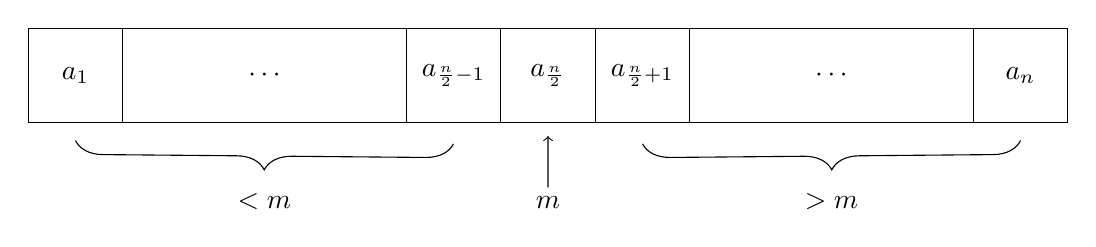
\begin{tikzpicture}[scale=1.2]

\draw (0,0) rectangle (1,1);
\node (a) at (0.5, 0.5) {$a_1$};

\draw (1,0) rectangle (4,1);
\node at (2.5, 0.5) {$\cdots$};

\draw (4,0) rectangle (5,1);
\node (b) at (4.5, 0.5) {$a_{\frac{n}{2}-1}$};

\draw (5,0) rectangle (6,1);
\node (am) at (5.5, 0.5) {$a_{\frac{n}{2}}$};

\draw (6,0) rectangle (7,1);
\node (c) at (6.5, 0.5) {$a_{\frac{n}{2}+1}$};

\draw (7,0) rectangle (10,1);
\node at (8.5, 0.5) {$\cdots$};

\draw (10,0) rectangle (11,1);
\node (d) at (10.5, 0.5) {$a_{n}$};


\node (m) at (5.5, -0.85) {$m$};
\draw[->,shorten >=0.5cm] (m) -- (am);


  \draw [decorate,decoration={brace,mirror,amplitude=10pt},xshift=-4pt,yshift=0pt] ([xshift=0cm,yshift=-.5cm]a.south) -- ([xshift=0cm,yshift=-0.5cm]b.south) node [black,midway,yshift=-0.75cm] {$< m$};

  \draw [decorate,decoration={brace,mirror,amplitude=10pt},xshift=-4pt,yshift=0pt] ([xshift=0cm,yshift=-.5cm]c.south) -- ([xshift=0cm,yshift=-0.5cm]d.south) node [black,midway,yshift=-0.75cm] {$> m$};


\end{tikzpicture}

%\caption[Array of Integers]{Array of Integers}
%\label{figure:arrayForSearching}
%\end{figure}
%
%\end{document}
%

\caption[A Sorted Array]{When an array is sorted, all elements in the left half are less than the middle element $m$, all elements in the
right half are greater than $m$.}
\label{figure:binarySearchDemo}
\end{figure}

Since the array is sorted, everything in the left-half 
of the array is $< m$ and everything in the right-half of the array 
is $> m$.\footnote{If duplicate elements
are in the array, then elements in the left/right half \emph{could}
be less than or equal to and greater than or equal to $m$, but this
will not affect how our algorithm works.}  We will now make one 
comparison between $e_k$ and $m$. There are three cases to consider.
\begin{enumerate}
  \item If $e_k = m$, then we've found \emph{an} element that matches
  	our key and search criteria and we are done.  We can output
	$m$ and stop the algorithm.
  \item If $e_k < m$ then we know that if a matching element exists, 
  	it must lie in the left-half of the list.  This is because all 
	elements in the right-half are $> m$.
  \item If $e_k > m$ then we know that if a matching element exists, 
  	it must lie in the right-half of the list.  This is because all 
	elements in the left-half are $< m$.
\end{enumerate}

In either of the second two cases, we have essentially cut the array
in half, halving the number of elements we need to consider.  Suppose
that the second case applies.  Then we can consider elements indexed
from $1$ to $\frac{n}{2}-1$ (we need not consider $a_{\frac{n}{2}}$ 
as the first case would have applied if we found a match).  We
can then do the same trick: check the middle element among the 
remaining elements and determine which half to cutout and which
half to consider.  We repeat this process until we've either found
the element we are looking for or the range in which we are searching
becomes ``empty'' indicating an unsuccessful search.

This description suggests a recursive solution.  Given two indices
$l, r$, we can compute the index of the middle element, $m = \frac{l + r}{2}$
and make one of two recursive calls depending on the cases identified
above.  Of course, we will need to make sure that our base case is taken
care of: if the two indices are \emph{invalid}, that is if the left
is greater than the right, $l > r$, then we know that the search
was unsuccessful.

\begin{algorithm}[H]
  \Input{A \emph{sorted} collection of elements $A = \{a_1, \ldots, a_n\}$, 
         bounds $1 \leq l, r \leq n$, and a key $e_k$}
  \Output{An element $a$ in $A$ such that $a = e_k$ according to some criteria; 
          $\phi$ if no such element exists}
  \If{$l > r$}{
    output $\phi$ \;
  }
  $m \leftarrow \lfloor \frac{l + r}{2} \rfloor$ \;
  \uIf{$a_m = e_k$}{ 
    output $a_m$ \;
  }
  \uElseIf{$a_m < e_k$}{ 
    \textsc{BinarySearch}$(A, m+1, r, e_k)$ \;
  }
  \Else{
    \textsc{BinarySearch}$(A, l, m-1, e_k)$ \;
  }
\caption{Recursive Binary Search Algorithm, $\textsc{BinarySearch}(A, l, r, e_k)$}
\label{algo:binarySearchRecursive}
\end{algorithm}

As discussed in Chapter \ref{chapter:recursion}, non-recursive solutions
are generally better than recursive ones.  We can design a straightforward
iterative version of binary search using a while loop.  We initialize two
index variables, $l, r$ and update them on each iteration depending on the
three cases above.  The loop stops when we've found our element or $l > r$
resulting in an unsuccessful search.  The iterative version is presented
in Algorithm \ref{algo:binarySearchIterative}, an example run of the
algorithm is shown in Figure \ref{figure:binarySearchExample}.

\begin{algorithm}[H]
  \Input{A \emph{sorted} collection of elements $A = \{a_1, \ldots, a_n\}$ 
         and a key $e_k$}
  \Output{An element $a \in A$ such that $a = e_k$ according to some criteria; 
          $\phi$ if no such element exists}
  $l \leftarrow 1$ \;
  $r \leftarrow n$ \;
  \While{$l \leq r$}{
    $m \leftarrow \lfloor \frac{l + r}{2} \rfloor$ \;
    \uIf{$a_m = e_k$}{ \label{algo:binarySearch:elemOp1}
      output $a_m$ \;
    }
    \uElseIf{$a_m < e_k$}{ \label{algo:binarySearch:elemOp2}
      $l \leftarrow (m+1)$ \;
    }
    \Else{
      $r \leftarrow (m-1)$ \;
    }
  }
  output $\phi$ \;
\caption{Iterative Binary Search Algorithm, $\textsc{BinarySearch}(A, e_k)$}
\label{algo:binarySearchIterative}
\end{algorithm}

%\documentclass[12pt]{scrbook}
%
%\usepackage{tikz}
%\usepackage{minted}
%\usetikzlibrary{decorations.pathreplacing}
%
%\usetikzlibrary{patterns}
%
%\usepackage{fullpage}
%\usepackage{subfigure}
%\begin{document}
%
%
%Lorem Ipsum is simply dummy text of the printing and typesetting industry. Lorem Ipsum has been the industry's standard dummy text ever since the 1500s, when an unknown printer took a galley of type and scrambled it to make a type specimen book. It has survived not only five centuries, but also the leap into electronic typesetting, remaining essentially unchanged. It was popularised in the 1960s with the release of Letraset sheets containing Lorem Ipsum passages, and more recently with desktop publishing software like Aldus PageMaker including versions of Lorem Ipsum.
%

\begin{figure}
\centering

\subfigure[Initially, $l = 0, r = 10$ and so we examine the middle
element at index $m = 5$ which is 12.]{

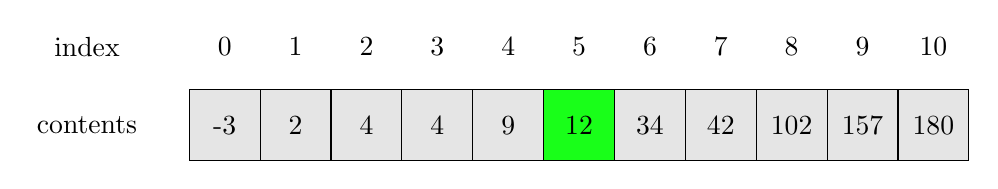
\begin{tikzpicture}
% size of each node
\def\sz{9mm}
% node style definition
\tikzstyle{block} = [
	draw, fill=black!10, rectangle,
	minimum height=\sz, minimum width=\sz ];
\tikzstyle{plain} = [draw=none,fill=none];
% array element definition
\def\arr{0, 2, 4, 4, 9, 12, 34, 42, 102};
%\def\x{0}; % x pos of arr
%\def\y{0}; % y pos of arr
%\newcounter{ind};
%\setcounter{ind}{0};
\node[plain] at (-1.75, 1) { index };
\node[plain] at (-1.75, 0) { contents };

\node[block] at (0,0) { -3 };
\node[plain] at (0,1.0) { 0 };

\node[block] at (1*\sz,0) { 2 };
\node[plain] at (1*\sz,1.0) { 1 };

\node[block] at (2*\sz,0) { 4 };
\node[plain] at (2*\sz,1.0) { 2 };

\node[block] at (3*\sz,0) { 4 };
\node[plain] at (3*\sz,1.0) { 3 };

\node[block] at (4*\sz,0) { 9 };
\node[plain] at (4*\sz,1.0) { 4 };

\node[block,fill=white!10!green] at (5*\sz,0) { 12 };
\node[plain] at (5*\sz,1.0) { 5 };

\node[block] at (6*\sz,0) { 34 };
\node[plain] at (6*\sz,1.0) { 6 };

\node[block] at (7*\sz,0) { 42 };
\node[plain] at (7*\sz,1.0) { 7 };

\node[block] at (8*\sz,0) { 102 };
\node[plain] at (8*\sz,1.0) { 8 };

\node[block] at (9*\sz,0) { 157 };
\node[plain] at (9*\sz,1.0) { 9 };

\node[block] at (10*\sz,0) { 180 };
\node[plain] at (10*\sz,1.0) { 10 };


%\foreach \item in \arr
%{
%	\node[block] (a\theind) at (\theind*\sz,0) { \item };
%	\node[plain] at (\theind*\sz,1.0) { \theind };
%	\addtocounter{ind}{1};
%}
\end{tikzpicture}

}

\subfigure[Since $64 > 12$, we update our left index variable
$l$ to $m + 1$, thus $l = 6$ and we've eliminated the left half
of the list from consideration.]{

\begin{tikzpicture}
% size of each node
\def\sz{9mm}
% node style definition
\tikzstyle{block} = [
	draw, fill=black!10, rectangle,
	minimum height=\sz, minimum width=\sz ];
\tikzstyle{plain} = [draw=none,fill=none];
% array element definition
\def\arr{0, 2, 4, 4, 9, 12, 34, 42, 102};
%\def\x{0}; % x pos of arr
%\def\y{0}; % y pos of arr
%\newcounter{ind};
%\setcounter{ind}{0};
\node[plain] at (-1.75, 1) { index };
\node[plain] at (-1.75, 0) { contents };

\node[block,pattern=north west lines, pattern color=blue] at (0,0) { -3 };
\node[plain] at (0,1.0) { 0 };

\node[block,pattern=north west lines, pattern color=blue] at (1*\sz,0) { 2 };
\node[plain] at (1*\sz,1.0) { 1 };

\node[block,pattern=north west lines, pattern color=blue] at (2*\sz,0) { 4 };
\node[plain] at (2*\sz,1.0) { 2 };

\node[block,pattern=north west lines, pattern color=blue] at (3*\sz,0) { 4 };
\node[plain] at (3*\sz,1.0) { 3 };

\node[block,pattern=north west lines, pattern color=blue] at (4*\sz,0) { 9 };
\node[plain] at (4*\sz,1.0) { 4 };

\node[block,fill=white!10!green] at (5*\sz,0) { 12 };
\node[plain] at (5*\sz,1.0) { 5 };

\node[block] at (6*\sz,0) { 34 };
\node[plain] at (6*\sz,1.0) { 6 };

\node[block] at (7*\sz,0) { 42 };
\node[plain] at (7*\sz,1.0) { 7 };

\node[block] at (8*\sz,0) { 102 };
\node[plain] at (8*\sz,1.0) { 8 };

\node[block] at (9*\sz,0) { 157 };
\node[plain] at (9*\sz,1.0) { 9 };

\node[block] at (10*\sz,0) { 180 };
\node[plain] at (10*\sz,1.0) { 10 };




%\foreach \item in \arr
%{
%	\node[block] (a\theind) at (\theind*\sz,0) { \item };
%	\node[plain] at (\theind*\sz,1.0) { \theind };
%	\addtocounter{ind}{1};
%}
\end{tikzpicture}

}



\subfigure[Our new middle index is $m = \frac{l+r}{2} = \frac{6+10}{2} = 8$, 
corresponding to the element 102.]{

\begin{tikzpicture}
% size of each node
\def\sz{9mm}
% node style definition
\tikzstyle{block} = [
	draw, fill=black!10, rectangle,
	minimum height=\sz, minimum width=\sz ];
\tikzstyle{plain} = [draw=none,fill=none];
% array element definition
\def\arr{0, 2, 4, 4, 9, 12, 34, 42, 102};
%\def\x{0}; % x pos of arr
%\def\y{0}; % y pos of arr
%\newcounter{ind};
%\setcounter{ind}{0};
\node[plain] at (-1.75, 1) { index };
\node[plain] at (-1.75, 0) { contents };

\node[block,pattern=north west lines, pattern color=blue] at (0,0) { -3 };
\node[plain] at (0,1.0) { 0 };

\node[block,pattern=north west lines, pattern color=blue] at (1*\sz,0) { 2 };
\node[plain] at (1*\sz,1.0) { 1 };

\node[block,pattern=north west lines, pattern color=blue] at (2*\sz,0) { 4 };
\node[plain] at (2*\sz,1.0) { 2 };

\node[block,pattern=north west lines, pattern color=blue] at (3*\sz,0) { 4 };
\node[plain] at (3*\sz,1.0) { 3 };

\node[block,pattern=north west lines, pattern color=blue] at (4*\sz,0) { 9 };
\node[plain] at (4*\sz,1.0) { 4 };

\node[block,pattern=north west lines, pattern color=blue] at (5*\sz,0) { 12 };
\node[plain] at (5*\sz,1.0) { 5 };

\node[block] at (6*\sz,0) { 34 };
\node[plain] at (6*\sz,1.0) { 6 };

\node[block] at (7*\sz,0) { 42 };
\node[plain] at (7*\sz,1.0) { 7 };

\node[block,fill=white!10!green] at (8*\sz,0) { 102 };
\node[plain] at (8*\sz,1.0) { 8 };

\node[block] at (9*\sz,0) { 157 };
\node[plain] at (9*\sz,1.0) { 9 };

\node[block] at (10*\sz,0) { 180 };
\node[plain] at (10*\sz,1.0) { 10 };




%\foreach \item in \arr
%{
%	\node[block] (a\theind) at (\theind*\sz,0) { \item };
%	\node[plain] at (\theind*\sz,1.0) { \theind };
%	\addtocounter{ind}{1};
%}
\end{tikzpicture}

}

\subfigure[Since $64 < 102$, we update the right index variable 
$r$ to $m - 1 = 7$, eliminating the right half of the subarray.]{

\begin{tikzpicture}
% size of each node
\def\sz{9mm}
% node style definition
\tikzstyle{block} = [
	draw, fill=black!10, rectangle,
	minimum height=\sz, minimum width=\sz ];
\tikzstyle{plain} = [draw=none,fill=none];
% array element definition
\def\arr{0, 2, 4, 4, 9, 12, 34, 42, 102};
%\def\x{0}; % x pos of arr
%\def\y{0}; % y pos of arr
%\newcounter{ind};
%\setcounter{ind}{0};
\node[plain] at (-1.75, 1) { index };
\node[plain] at (-1.75, 0) { contents };

\node[block,pattern=north west lines, pattern color=blue] at (0,0) { -3 };
\node[plain] at (0,1.0) { 0 };

\node[block,pattern=north west lines, pattern color=blue] at (1*\sz,0) { 2 };
\node[plain] at (1*\sz,1.0) { 1 };

\node[block,pattern=north west lines, pattern color=blue] at (2*\sz,0) { 4 };
\node[plain] at (2*\sz,1.0) { 2 };

\node[block,pattern=north west lines, pattern color=blue] at (3*\sz,0) { 4 };
\node[plain] at (3*\sz,1.0) { 3 };

\node[block,pattern=north west lines, pattern color=blue] at (4*\sz,0) { 9 };
\node[plain] at (4*\sz,1.0) { 4 };

\node[block,pattern=north west lines, pattern color=blue] at (5*\sz,0) { 12 };
\node[plain] at (5*\sz,1.0) { 5 };

\node[block] at (6*\sz,0) { 34 };
\node[plain] at (6*\sz,1.0) { 6 };

\node[block] at (7*\sz,0) { 42 };
\node[plain] at (7*\sz,1.0) { 7 };

\node[block,fill=white!10!green] at (8*\sz,0) { 102 };
\node[plain] at (8*\sz,1.0) { 8 };

\node[block,pattern=north west lines, pattern color=blue] at (9*\sz,0) { 157 };
\node[plain] at (9*\sz,1.0) { 9 };

\node[block,pattern=north west lines, pattern color=blue] at (10*\sz,0) { 180 };
\node[plain] at (10*\sz,1.0) { 10 };




%\foreach \item in \arr
%{
%	\node[block] (a\theind) at (\theind*\sz,0) { \item };
%	\node[plain] at (\theind*\sz,1.0) { \theind };
%	\addtocounter{ind}{1};
%}
\end{tikzpicture}

}


\subfigure[Here, $l = 6, r = 7$, and so our new middle index is
$m = \lfloor \frac{6 + 7}{2}\rfloor = 6$.  Since $64 > 34$, we 
update our left index variable $l$ to $m+1 = 7$]{

\begin{tikzpicture}
% size of each node
\def\sz{9mm}
% node style definition
\tikzstyle{block} = [
	draw, fill=black!10, rectangle,
	minimum height=\sz, minimum width=\sz ];
\tikzstyle{plain} = [draw=none,fill=none];
% array element definition
\def\arr{0, 2, 4, 4, 9, 12, 34, 42, 102};
%\def\x{0}; % x pos of arr
%\def\y{0}; % y pos of arr
%\newcounter{ind};
%\setcounter{ind}{0};
\node[plain] at (-1.75, 1) { index };
\node[plain] at (-1.75, 0) { contents };

\node[block,pattern=north west lines, pattern color=blue] at (0,0) { -3 };
\node[plain] at (0,1.0) { 0 };

\node[block,pattern=north west lines, pattern color=blue] at (1*\sz,0) { 2 };
\node[plain] at (1*\sz,1.0) { 1 };

\node[block,pattern=north west lines, pattern color=blue] at (2*\sz,0) { 4 };
\node[plain] at (2*\sz,1.0) { 2 };

\node[block,pattern=north west lines, pattern color=blue] at (3*\sz,0) { 4 };
\node[plain] at (3*\sz,1.0) { 3 };

\node[block,pattern=north west lines, pattern color=blue] at (4*\sz,0) { 9 };
\node[plain] at (4*\sz,1.0) { 4 };

\node[block,pattern=north west lines, pattern color=blue] at (5*\sz,0) { 12 };
\node[plain] at (5*\sz,1.0) { 5 };

\node[block,fill=white!10!green] at (6*\sz,0) { 34 };
\node[plain] at (6*\sz,1.0) { 6 };

\node[block] at (7*\sz,0) { 42 };
\node[plain] at (7*\sz,1.0) { 7 };

\node[block,pattern=north west lines, pattern color=blue] at (8*\sz,0) { 102 };
\node[plain] at (8*\sz,1.0) { 8 };

\node[block,pattern=north west lines, pattern color=blue] at (9*\sz,0) { 157 };
\node[plain] at (9*\sz,1.0) { 9 };

\node[block,pattern=north west lines, pattern color=blue] at (10*\sz,0) { 180 };
\node[plain] at (10*\sz,1.0) { 10 };




%\foreach \item in \arr
%{
%	\node[block] (a\theind) at (\theind*\sz,0) { \item };
%	\node[plain] at (\theind*\sz,1.0) { \theind };
%	\addtocounter{ind}{1};
%}
\end{tikzpicture}

}

\subfigure[Since $64 > 42$ we again update our left index variable $l$
to $m + 1 = 8$.]{

\begin{tikzpicture}
% size of each node
\def\sz{9mm}
% node style definition
\tikzstyle{block} = [
	draw, fill=black!10, rectangle,
	minimum height=\sz, minimum width=\sz ];
\tikzstyle{plain} = [draw=none,fill=none];
% array element definition
\def\arr{0, 2, 4, 4, 9, 12, 34, 42, 102};
%\def\x{0}; % x pos of arr
%\def\y{0}; % y pos of arr
%\newcounter{ind};
%\setcounter{ind}{0};
\node[plain] at (-1.75, 1) { index };
\node[plain] at (-1.75, 0) { contents };

\node[block,pattern=north west lines, pattern color=blue] at (0,0) { -3 };
\node[plain] at (0,1.0) { 0 };

\node[block,pattern=north west lines, pattern color=blue] at (1*\sz,0) { 2 };
\node[plain] at (1*\sz,1.0) { 1 };

\node[block,pattern=north west lines, pattern color=blue] at (2*\sz,0) { 4 };
\node[plain] at (2*\sz,1.0) { 2 };

\node[block,pattern=north west lines, pattern color=blue] at (3*\sz,0) { 4 };
\node[plain] at (3*\sz,1.0) { 3 };

\node[block,pattern=north west lines, pattern color=blue] at (4*\sz,0) { 9 };
\node[plain] at (4*\sz,1.0) { 4 };

\node[block,pattern=north west lines, pattern color=blue] at (5*\sz,0) { 12 };
\node[plain] at (5*\sz,1.0) { 5 };

\node[block,pattern=north west lines, pattern color=blue] at (6*\sz,0) { 34 };
\node[plain] at (6*\sz,1.0) { 6 };

\node[block,fill=white!10!green] at (7*\sz,0) { 42 };
\node[plain] at (7*\sz,1.0) { 7 };

\node[block,pattern=north west lines, pattern color=blue] at (8*\sz,0) { 102 };
\node[plain] at (8*\sz,1.0) { 8 };

\node[block,pattern=north west lines, pattern color=blue] at (9*\sz,0) { 157 };
\node[plain] at (9*\sz,1.0) { 9 };

\node[block,pattern=north west lines, pattern color=blue] at (10*\sz,0) { 180 };
\node[plain] at (10*\sz,1.0) { 10 };




%\foreach \item in \arr
%{
%	\node[block] (a\theind) at (\theind*\sz,0) { \item };
%	\node[plain] at (\theind*\sz,1.0) { \theind };
%	\addtocounter{ind}{1};
%}
\end{tikzpicture}

}

\subfigure[Since $l = 8$ and $r = 7$, $l > r$ and the loop terminates, 
resulting in an unsuccessful search.]{

\begin{tikzpicture}
% size of each node
\def\sz{9mm}
% node style definition
\tikzstyle{block} = [
	draw, fill=black!10, rectangle,
	minimum height=\sz, minimum width=\sz ];
\tikzstyle{plain} = [draw=none,fill=none];
% array element definition
\def\arr{0, 2, 4, 4, 9, 12, 34, 42, 102};
%\def\x{0}; % x pos of arr
%\def\y{0}; % y pos of arr
%\newcounter{ind};
%\setcounter{ind}{0};
\node[plain] at (-1.75, 1) { index };
\node[plain] at (-1.75, 0) { contents };

\node[block,pattern=north west lines, pattern color=blue] at (0,0) { -3 };
\node[plain] at (0,1.0) { 0 };

\node[block,pattern=north west lines, pattern color=blue] at (1*\sz,0) { 2 };
\node[plain] at (1*\sz,1.0) { 1 };

\node[block,pattern=north west lines, pattern color=blue] at (2*\sz,0) { 4 };
\node[plain] at (2*\sz,1.0) { 2 };

\node[block,pattern=north west lines, pattern color=blue] at (3*\sz,0) { 4 };
\node[plain] at (3*\sz,1.0) { 3 };

\node[block,pattern=north west lines, pattern color=blue] at (4*\sz,0) { 9 };
\node[plain] at (4*\sz,1.0) { 4 };

\node[block,pattern=north west lines, pattern color=blue] at (5*\sz,0) { 12 };
\node[plain] at (5*\sz,1.0) { 5 };

\node[block,pattern=north west lines, pattern color=blue] at (6*\sz,0) { 34 };
\node[plain] at (6*\sz,1.0) { 6 };

\node[block,pattern=north west lines, pattern color=blue] at (7*\sz,0) { 42 };
\node[plain] at (7*\sz,1.0) { 7 };

\node[block,pattern=north west lines, pattern color=blue] at (8*\sz,0) { 102 };
\node[plain] at (8*\sz,1.0) { 8 };

\node[block,pattern=north west lines, pattern color=blue] at (9*\sz,0) { 157 };
\node[plain] at (9*\sz,1.0) { 9 };

\node[block,pattern=north west lines, pattern color=blue] at (10*\sz,0) { 180 };
\node[plain] at (10*\sz,1.0) { 10 };




%\foreach \item in \arr
%{
%	\node[block] (a\theind) at (\theind*\sz,0) { \item };
%	\node[plain] at (\theind*\sz,1.0) { \theind };
%	\addtocounter{ind}{1};
%}
\end{tikzpicture}

}

\caption[Binary Search Example]{The worst case scenario for binary search, 
resulting in an unsuccessful search for $e_k=64$.  This example is run on a 0-indexed array
with an array of integers of size 11.}
\label{figure:binarySearchExample}

\end{figure}




%\end{document}


\subsection{Analysis}
\index{search algorithm!analysis}

When algorithms are implemented and run on a computer, they require a
certain amount of \emph{resources}.  In general, we could consider a lot
of different resources such as computation time and memory.  Algorithm
analysis involves quantifying how many resource(s) an algorithm requires
to execute with respect to the size of the input it is run on.

When analyzing algorithms, we want to keep the analysis as abstract and 
general as possible, independent of any particular language, framework or
hardware.  We could always update the hardware on which we run our implementation, 
but that does not necessarily make the \index{algorithm} 
\emph{algorithm} faster.  The algorithm would still execute the same
\emph{number} of operations.  Faster machines just mean that more
steps can be performed in less time.  In
fact, the concept of an algorithm itself is a mathematical concept that
predates modern computers by thousands of years.  One of the oldest algorithms,
for example, Euler's GCD (greatest common divisor) algorithm dates to 300
BCE.  Whether or not you're ``running'' it on a piece of papyrus 2,300 years
ago or on a modern supercomputer, the same number of divisions and subtractions
are performed.

To keep things abstract, we analyze an algorithm by identifying
an \index{elementary operation} \emph{elementary operation}.  This is generally the most common or most
``expensive'' operation that the algorithm performs.  Sometimes there may be more
than one reasonable choice for an elementary operation which may give different results in our analysis.  However, we generally do \emph{not} consider basic operations
that are necessary to the \emph{control flow} of an algorithm.  For example, 
variable assignments or the iteration of index variables.

Once we have identified an elementary operation, we can quantify the complexity
of an algorithm by analyzing the number of times the elementary operation is
executed with respect to the \emph{input size}.  For a collection, the input
size is generally the number of elements in the collection, $n$.  We can
then characterize the number of elementary operations and thus the complexity
of the algorithm itself as a \emph{function} of the input size.  We illustrate
this process by analyzing and comparing the two search algorithms.

\subsubsection{Linear Search Analysis}

When considering the linear search algorithm, the input size is clearly the
number of elements in the collection, $n$.  The best candidate for the
elementary operation is the comparison (Line \ref{algo:linearSearch:elemOp}, 
Algorithm \ref{algo:linearSearch}).  To analyze this algorithm, we need
to determine how many comparisons are made with respect to the size of
the collection, $n$.

As we saw in the examples, the number of comparisons made by linear search
can vary depending on the element we're searching and the configuration of
the collection being searched.  Because of this variability, we can 
analyze the algorithm in one of three ways: by looking at the best case
scenario, worst case scenario, and average case scenario.

The best case scenario is when the number of operations is \emph{minimized}.
For linear search, the best case scenario happens when we get lucky and
the first element that we examine matches our criteria, requiring only a 
single comparison operation.  In general, it is not reasonable to assume
that the best case scenario will be commonly encountered.

The worst case scenario is when the number of operations is \emph{maximized}.
This happens when we get ``unlucky'' and have to search the entire collection
finding a match at the last element or not finding a match at all.  In either
case, we make $n$ comparisons to search the collection.

A formal average case analysis is not difficult, but is a bit beyond the
scope of the present analysis.  However, informally, we could expect to make
about $\frac{n}{2}$ comparisons for successful searches if we assume that
all elements have a uniform probability of being searched for.

Both the worst-case and average-case are reasonable scenarios from which to
analyze the linear search algorithm.  In the end, however, the only difference
between the two analyses is a constant factor.  Both analyses result in two
linear functions, 
  $$f_1(n) = n \quad f_2(n) = \frac{1}{2}n$$
The only difference being the constant factor $\frac{1}{2}$.  In fact, this
is why the algorithm is called \emph{linear} search.  The number of comparison
operations performed by the algorithm \emph{grows linearly} with respect
to the input size.  For example, if we were to double the input size from
$n$ to $2n$, then we would expect the number of comparisons to search the
collection would also double (this applies in either the worst-case and average-case
scenarios).  This is what is most important in algorithm analysis: quantifying
the complexity of an algorithm by the rate of growth of the operations (and
thus resources) required to execute the algorithm as the input size $n$ 
grows.\footnote{This is the basis of Big-O analysis, something that 
we will not discuss in detail here, but is of prime importance when analyzing
algorithms.}

\subsubsection{Binary Search Analysis}
\index{binary search!analysis}

Like linear search, the input size is the size of the collection $n$ and the
elementary operation is the comparison.  As presented in the pseudocode, 
binary search would seem to perform \emph{two} comparisons (Lines
\ref{algo:binarySearch:elemOp1} and \ref{algo:binarySearch:elemOp2} in Algorithm
\ref{algo:binarySearchIterative}).  However, to make the analysis simpler, we
will instead count one comparison operation per iteration of the 
while loop.  This is a reasonable simplification; in practice the comparison
operation would likely involve a single function call, after which 
distinguishing between the three cases is a simple matter of control flow.
Further, even if we were to consider both comparisons, it would only contribute
a constant factor of 2 to the final analysis.

Since we perform one comparison for each iteration of the while loop, we need
to determine how many times the while loop executes.  In the worst case, the
number of iterations is maximized when we fail to find an element that does
not match our criteria.  However each iteration essentially cuts the array in
half each time.  That is, if we start with an array of size $n$, then after the 
first iteration, it is of size $\frac{n}{2}$.  After the second iteration
we have cut it in half again, so it is of size $\frac{n}{4}$, after the third
iteration it is of size $\frac{n}{8}$ and so on.  More generally, after
$k$ iterations, the size of the array is
  $$\frac{n}{2^k}$$
The loop terminates one iteration \emph{after} the the index variables are 
equal, $l = r$.  Equivalently, when $l = r$, the size of the subarray under consideration is 1.  That is, the algorithm stops when the array size has
been cut down to 1:
  $$\frac{n}{2^k} = 1$$
Solving for $k$ gives us the number of iterations:
  $$k = \log_2{(n)}$$
Adding one additional comparison for the final iteration gives us a
total of 
  $$k = \log_2{(n)}$$
comparisons (see Table \ref{table:binarySearchComparisons}).  Thus, binary search performs a logarithmic number of 
comparisons in the worst
case.  As we will see, this is \emph{exponentially} better than linear search.

{\renewcommand{\arraystretch}{1.5}
\begin{table}[h]
\centering
\begin{tabular}{c|c|c}
Iteration & Array Size & Comparisons \\
\hline\hline
1 & $\frac{n}{2}$ & 1 \\
2 & $\frac{n}{4}$ & 1 \\
3 & $\frac{n}{8}$ & 1 \\
4 & $\frac{n}{16}$ & 1 \\
\vdots & \vdots & \vdots \\
$k$ & $\frac{n}{2^k}$ & 1 \\
\vdots & \vdots & \vdots \\
$\log_2{(n)}$ & 1 & 1 \\
$\log_2{(n)}+1$ & 0 & 1 \\
\hline
\multicolumn{2}{c|}{Total} & $\log_2{(n)} + 1$ \\
\end{tabular}
\caption[Binary Search Comparison Total]{Number of comparisons and array size 
after the iteration during the execution of binary search.}
\label{table:binarySearchComparisons}
\end{table}
}

\subsubsection{Comparative Analysis}

Binary search presents a clear advantage over linear search.  There is
an \emph{exponential} difference between a linear function, $\frac{n}{2}$
and a logarithmic function, $\log_2{(n)}$.  To put this in
perspective, consider searching a \emph{moderately} large database of 1
trillion ($10^{12}$) records.\footnote{In the era of ``big data,'' 1 trillion
records only qualifies as \emph{moderately} large.}  Using linear search, 
even the average-case scenario would require about
  $$\frac{10^{12}}{2} = 5 \times 10^{11}$$
or about 500 billion comparisons.  However, using binary search would only
require at most 
  $$\log_2{(10^{12})} = 12 \cdot \log_2{(10)} < 40$$ 
comparisons to search.  This is a \emph{huge} difference in performance.

As another comparison, let's consider how each algorithm's complexity
grows as we increase the size of the collection being searched.  As observed
earlier, if we double the input size, $n \rightarrow 2n$, we would expect
the number of comparisons performed by linear search to also double.
However, if we double the input size for binary search, we get the following.
  $$\log_2{(2n)} = \log_2{(2)} + \log{(n)} = \log{(n)} + 1$$
That is, only a single additional comparison is necessary to search an array
of twice the size.

The difference between these two algorithms shows up in many different instances.
Figure \ref{figure:windows7Example} contains a screen shot of the search feature
in Windows 7.  When searching for particular files or content in particular files,
the search can be greatly increased if the files have been \emph{indexed}, that
is, sorted.  As the dialog indicates, non-indexed (unsorted) records will take
far longer to search.

\begin{figure}[h]
\centering
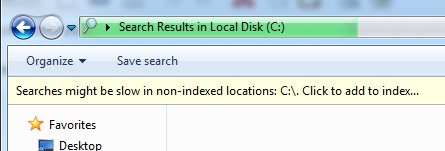
\includegraphics[scale=0.5]{images/windows7Example}
\caption{Example of the benefit of ordered (indexed) elements in Windows 7}
\label{figure:windows7Example}
\end{figure}

Though binary search presents a clear advantage over linear search, it only works
if the collection has been sorted.\footnote{Binary search also only works when
searching an array with random access to its elements.  The performance of binary
search cannot generally be realized with data structures such as linked lists or 
unordered sets.}  Thus, we now turn our attention to the problem of sorting
a collection.

\section{Sorting}
\index{sorting}

Sorting a collection of data is another fundamental data operation.  It is
conceptually simple, but is ubiquitous.  There are a large variety of
algorithms, data structures and applications built around the problem
of sorting.  As we've already seen, being able to sort a collection provides 
a huge speed up when searching for a particular element.  Sorting provides 
a natural way to store and organize data.  

\begin{problem}[Sorting]
~\\
\textbf{Given:} a collection of \emph{orderable} elements, $A =\{a_1, a_2, \ldots, a_n\}$\\
\textbf{Output:} $A$, sorted in ascending order
\end{problem}

The requirement that the collection be made of ``orderable'' elements can be
a bit technical\footnote{We require that $A$ be a \emph{total order} a 
partially ordered binary relation such that all pairs are comparable.}, but essentially 
we need to be guaranteed that given two elements, $a, b$ in the collection, 
we can determine whether $a < b$, $a = b$ or $a > b$.  If such a determination
cannot be made, then sorting is impossible.

Again, we can consider variations on this problem.  We may want our collection
to be sorted in descending order instead of ascending.\footnote{Technically, these are
referred to as \emph{non-decreasing} and \emph{non-increasing} respectively.  
This is because the collection could contain duplicate elements and not lead
to a strictly increasing or strictly decreasing ordering.} We may also want
the collection itself to be \emph{permuted} (that is, reordered) or we may
instead want a \emph{copy} of the collection to be created and sorted so that
the original is unchanged.

We will examine several standard sorting algorithms. Though there are dozens
of sorting algorithms, we will only focus on a few of the more common ones.  
As with 
searching, we can analyze a sorting algorithm based on the number of 
comparisons it makes in the worst, best, or average cases.  We may also look
at alternative resources or operations: how many swaps does the algorithm make?
How much extra memory is required?  Etc.

Though we will examine, analyze and compare several sorting algorithms, most
programming languages provide standard functionality to sort a collection of
elements.  It is generally preferable to use the functionality built into 
whatever language you're using rather that reimplementing your own.  Typically, 
these functions are well-designed, well-tested, optimized and more efficient
than any custom alternatives.

\subsection{Selection Sort}
\index{Selection Sort}
\index{sorting!Selection Sort}

The first sorting algorithm we'll examine is \emph{Selection Sort} which is
similar to the way a human would sort a collection of objects.  The basic idea
is that you search through the collection and find the minimal element 
(we say minimal and not minimum because there could be elements with the
same value).  Once we've found a minimal element, we can swap it with the
``first'' element, $a_1$, placing the minimal element where it belongs in
the collection.  

We repeat this process for the remaining elements, $a_2, \ldots, a_n$, 
finding the minimal element among these and swapping with $a_2$.  In 
general, if we have already sorted the first $i-1$ elements, 
$a_1, \ldots, a_{i-1}$ then we only need to examine the elements
$a_i, \ldots, a_n$ for the minimal element, swapping it with $a_i$.
We end this process after we have sorted the first $n-1$ elements, 
$a_1, \ldots, a_{n-1}$ since the last element $a_n$ will already
be where it needs to be.  We present Selection Sort as Algorithm 
\ref{algo:selectionSort}.  We illustrate the execution of Selection 
Sort in Figure \ref{figure:selectionSortExample}. 

    \begin{algorithm}[H]
     \Input{A collection $A = \{a_1, \ldots, a_n\}$}
     \Output{An array $A'$ containing all elements of $A$ in nondecreasing order}
     \For{$i = 1, \ldots, (n-1)$}{
       $a_{min} \leftarrow a_i$ \;
       \For{$j = (i+1), \ldots, n$}{
         \If{$a_{min} > a_j$}{ \label{algo:selectionSortComp}
           $min \leftarrow a_j$ \;
         }
       }
       swap $a_{min}$ and $a_i$ \;
     }
    \caption{Selection Sort}
    \label{algo:selectionSort}
    \end{algorithm}

%\documentclass[12pt]{scrbook}
%
%\usepackage{tikz}
%\usepackage{minted}
%\usetikzlibrary{decorations.pathreplacing,arrows}
%\usetikzlibrary{arrows,decorations.pathmorphing,backgrounds,positioning,fit,petri}
%
%\usepackage{fullpage}
%\usepackage{subfigure}
%\begin{document}
%
%
%Lorem Ipsum is simply dummy text of the printing and typesetting industry. Lorem Ipsum has been the industry's standard dummy text ever since the 1500s, when an unknown printer took a galley of type and scrambled it to make a type specimen book. It has survived not only five centuries, but also the leap into electronic typesetting, remaining essentially unchanged. It was popularised in the 1960s with the release of Letraset sheets containing Lorem Ipsum passages, and more recently with desktop publishing software like Aldus PageMaker including versions of Lorem Ipsum.
%




\begin{figure}
\centering

\subfigure[First iteration.  We find the minimal element, 0, at the last
index, swapping it with the first element.  At this point, the first
element is sorted.]{

\begin{tikzpicture}[scale=.65,transform shape]

\tikzset{>=stealth',shorten <=.2cm,>=stealth',shorten >=.2cm}
% size of each node
\def\sz{9mm}
% node style definition
\tikzstyle{block} = [
	draw, fill=black!10, rectangle,
	minimum height=\sz, minimum width=\sz ];
\tikzstyle{plain} = [draw=none,fill=none];

%\node[plain] at (-1.75, 1) { index };
%\node[plain] at (0*\sz,1.0) { 0 };
%\node[plain] at (1*\sz,1.0) { 1 };
%\node[plain] at (2*\sz,1.0) { 2 };
%\node[plain] at (3*\sz,1.0) { 3 };
%\node[plain] at (4*\sz,1.0) { 4 };
%\node[plain] at (5*\sz,1.0) { 5 };
%\node[plain] at (6*\sz,1.0) { 6 };
%\node[plain] at (7*\sz,1.0) { 7 };
%\node[plain] at (8*\sz,1.0) { 8 };
%\node[plain] at (-1.75, 0) { contents };
%

\node[block,fill=black!30] (a0) at (0*\sz,0) { 42 };
\node[block] (a1) at (1*\sz,0) { 4 };
\node[block] (a2) at (2*\sz,0) { 9 };
\node[block] (a3) at (3*\sz,0) { 4 };
\node[block] (a4) at (4*\sz,0) { 102 };
\node[block] (a5) at (5*\sz,0) { 34 };
\node[block] (a6) at (6*\sz,0) { 12 };
\node[block] (a7) at (7*\sz,0) { 2 };
\node[block,fill=green!30] (a8) at (8*\sz,0) { 0 };

\draw[<->] (a0.south) to [bend right] node[pos=.5,below] {swap} (a8.south);

\end{tikzpicture}~~~~~\begin{tikzpicture}[scale=.65,transform shape]
\draw[white] (0,0) rectangle (1, -2.05);

\tikzset{>=stealth',shorten <=.2cm,>=stealth',shorten >=.2cm}
\def\sz{9mm}
\tikzstyle{block} = [
	draw, fill=black!10, rectangle,
	minimum height=\sz, minimum width=\sz ];
\tikzstyle{plain} = [draw=none,fill=none];

\node[block,fill=black!50] (a0) at (0*\sz,0) { 0 };
\node[block] (a1) at (1*\sz,0) { 4 };
\node[block] (a2) at (2*\sz,0) { 9 };
\node[block] (a3) at (3*\sz,0) { 4 };
\node[block] (a4) at (4*\sz,0) { 102 };
\node[block] (a5) at (5*\sz,0) { 34 };
\node[block] (a6) at (6*\sz,0) { 12 };
\node[block] (a7) at (7*\sz,0) { 2 };
\node[block] (a8) at (8*\sz,0) { 42 };

\end{tikzpicture}

}

\subfigure[Second Iteration.  Now starting with the second element, the
minimal element among the remaining is found at the second to last element.
4 and 2 are swapped.  At this point, the first two elements are sorted.]{

\begin{tikzpicture}[scale=.65,transform shape]

\tikzset{>=stealth',shorten <=.2cm,>=stealth',shorten >=.2cm}
\def\sz{9mm}
\tikzstyle{block} = [
	draw, fill=black!10, rectangle,
	minimum height=\sz, minimum width=\sz ];
\tikzstyle{plain} = [draw=none,fill=none];

\node[block,fill=black!50] (a0) at (0*\sz,0) { 0 };
\node[block,fill=black!30] (a1) at (1*\sz,0) { 4 };
\node[block] (a2) at (2*\sz,0) { 9 };
\node[block] (a3) at (3*\sz,0) { 4 };
\node[block] (a4) at (4*\sz,0) { 102 };
\node[block] (a5) at (5*\sz,0) { 34 };
\node[block] (a6) at (6*\sz,0) { 12 };
\node[block,fill=green!30] (a7) at (7*\sz,0) { 2 };
\node[block] (a8) at (8*\sz,0) { 42 };

\draw[<->] (a1.south) to [bend right] node[pos=.5,below] {swap} (a7.south);

\end{tikzpicture}~~~~~\begin{tikzpicture}[scale=.65,transform shape]
\draw[white] (0,0) rectangle (1, -1.75);

\tikzset{>=stealth',shorten <=.2cm,>=stealth',shorten >=.2cm}
\def\sz{9mm}
\tikzstyle{block} = [
	draw, fill=black!10, rectangle,
	minimum height=\sz, minimum width=\sz ];
\tikzstyle{plain} = [draw=none,fill=none];

\node[block,fill=black!50] (a0) at (0*\sz,0) { 0 };
\node[block,fill=black!50] (a1) at (1*\sz,0) { 2 };
\node[block] (a2) at (2*\sz,0) { 9 };
\node[block] (a3) at (3*\sz,0) { 4 };
\node[block] (a4) at (4*\sz,0) { 102 };
\node[block] (a5) at (5*\sz,0) { 34 };
\node[block] (a6) at (6*\sz,0) { 12 };
\node[block] (a7) at (7*\sz,0) { 4 };
\node[block] (a8) at (8*\sz,0) { 42 };

%\draw[<->] (a1.south) to [bend right] node[pos=.5,below] {swap} (a7.south);

\end{tikzpicture}

}

\subfigure[Third iteration.  Since we are using the strictly-less than comparison, the first 4 is the minimal element and swapped with 9.]{

\begin{tikzpicture}[scale=.65,transform shape]

\tikzset{>=stealth',shorten <=.2cm,>=stealth',shorten >=.2cm}
\def\sz{9mm}
\tikzstyle{block} = [
	draw, fill=black!10, rectangle,
	minimum height=\sz, minimum width=\sz ];
\tikzstyle{plain} = [draw=none,fill=none];

\node[block,fill=black!50] (a0) at (0*\sz,0) { 0 };
\node[block,fill=black!50] (a1) at (1*\sz,0) { 2 };
\node[block,fill=black!30] (a2) at (2*\sz,0) { 9 };
\node[block,fill=green!30] (a3) at (3*\sz,0) { 4 };
\node[block] (a4) at (4*\sz,0) { 102 };
\node[block] (a5) at (5*\sz,0) { 34 };
\node[block] (a6) at (6*\sz,0) { 12 };
\node[block] (a7) at (7*\sz,0) { 4 };
\node[block] (a8) at (8*\sz,0) { 42 };

\draw[<->] (a2.south) to [bend right] node[pos=.5,below] {swap} (a3.south);

\end{tikzpicture}~~~~~\begin{tikzpicture}[scale=.65,transform shape]
\draw[white] (0,0) rectangle (1, -1.1);

\tikzset{>=stealth',shorten <=.2cm,>=stealth',shorten >=.2cm}
\def\sz{9mm}
\tikzstyle{block} = [
	draw, fill=black!10, rectangle,
	minimum height=\sz, minimum width=\sz ];
\tikzstyle{plain} = [draw=none,fill=none];

\node[block,fill=black!50] (a0) at (0*\sz,0) { 0 };
\node[block,fill=black!50] (a1) at (1*\sz,0) { 2 };
\node[block,fill=black!50] (a2) at (2*\sz,0) { 4 };
\node[block] (a3) at (3*\sz,0) { 9 };
\node[block] (a4) at (4*\sz,0) { 102 };
\node[block] (a5) at (5*\sz,0) { 34 };
\node[block] (a6) at (6*\sz,0) { 12 };
\node[block] (a7) at (7*\sz,0) { 4 };
\node[block] (a8) at (8*\sz,0) { 42 };

%\draw[<->] (a1.south) to [bend right] node[pos=.5,below] {swap} (a7.south);

\end{tikzpicture}

}

\subfigure[Fourth iteration.  At this point, the first 3 elements are
sorted.  We find the minimal element (the other 4) and swap it with
9.  At the end of this iteration, the first 4 elements are sorted.]{

\begin{tikzpicture}[scale=.65,transform shape]

\tikzset{>=stealth',shorten <=.2cm,>=stealth',shorten >=.2cm}
\def\sz{9mm}
\tikzstyle{block} = [
	draw, fill=black!10, rectangle,
	minimum height=\sz, minimum width=\sz ];
\tikzstyle{plain} = [draw=none,fill=none];

\node[block,fill=black!50] (a0) at (0*\sz,0) { 0 };
\node[block,fill=black!50] (a1) at (1*\sz,0) { 2 };
\node[block,fill=black!50] (a2) at (2*\sz,0) { 4 };
\node[block,fill=black!30] (a3) at (3*\sz,0) { 9 };
\node[block] (a4) at (4*\sz,0) { 102 };
\node[block] (a5) at (5*\sz,0) { 34 };
\node[block] (a6) at (6*\sz,0) { 12 };
\node[block,fill=green!30] (a7) at (7*\sz,0) { 4 };
\node[block] (a8) at (8*\sz,0) { 42 };

\draw[<->] (a3.south) to [bend right] node[pos=.5,below] {swap} (a7.south);

\end{tikzpicture}~~~~~\begin{tikzpicture}[scale=.65,transform shape]
\draw[white] (0,0) rectangle (1, -1.5);

\tikzset{>=stealth',shorten <=.2cm,>=stealth',shorten >=.2cm}
\def\sz{9mm}
\tikzstyle{block} = [
	draw, fill=black!10, rectangle,
	minimum height=\sz, minimum width=\sz ];
\tikzstyle{plain} = [draw=none,fill=none];

\node[block,fill=black!50] (a0) at (0*\sz,0) { 0 };
\node[block,fill=black!50] (a1) at (1*\sz,0) { 2 };
\node[block,fill=black!50] (a2) at (2*\sz,0) { 4 };
\node[block,fill=black!50] (a3) at (3*\sz,0) { 4 };
\node[block] (a4) at (4*\sz,0) { 102 };
\node[block] (a5) at (5*\sz,0) { 34 };
\node[block] (a6) at (6*\sz,0) { 12 };
\node[block] (a7) at (7*\sz,0) { 9 };
\node[block] (a8) at (8*\sz,0) { 42 };

%\draw[<->] (a1.south) to [bend right] node[pos=.5,below] {swap} (a7.south);

\end{tikzpicture}

}

\subfigure[Fifth iteration.  The 9 is swapped with 102, sorting
the first 5 elements.]{

\begin{tikzpicture}[scale=.65,transform shape]

\tikzset{>=stealth',shorten <=.2cm,>=stealth',shorten >=.2cm}
\def\sz{9mm}
\tikzstyle{block} = [
	draw, fill=black!10, rectangle,
	minimum height=\sz, minimum width=\sz ];
\tikzstyle{plain} = [draw=none,fill=none];

\node[block,fill=black!50] (a0) at (0*\sz,0) { 0 };
\node[block,fill=black!50] (a1) at (1*\sz,0) { 2 };
\node[block,fill=black!50] (a2) at (2*\sz,0) { 4 };
\node[block,fill=black!50] (a3) at (3*\sz,0) { 4 };
\node[block,fill=black!30] (a4) at (4*\sz,0) { 102 };
\node[block] (a5) at (5*\sz,0) { 34 };
\node[block] (a6) at (6*\sz,0) { 12 };
\node[block,fill=green!30] (a7) at (7*\sz,0) { 9 };
\node[block] (a8) at (8*\sz,0) { 42 };

\draw[<->] (a4.south) to [bend right] node[pos=.5,below] {swap} (a7.south);

\end{tikzpicture}~~~~~\begin{tikzpicture}[scale=.65,transform shape]
\draw[white] (0,0) rectangle (1, -1.4);

\tikzset{>=stealth',shorten <=.2cm,>=stealth',shorten >=.2cm}
\def\sz{9mm}
\tikzstyle{block} = [
	draw, fill=black!10, rectangle,
	minimum height=\sz, minimum width=\sz ];
\tikzstyle{plain} = [draw=none,fill=none];

\node[block,fill=black!50] (a0) at (0*\sz,0) { 0 };
\node[block,fill=black!50] (a1) at (1*\sz,0) { 2 };
\node[block,fill=black!50] (a2) at (2*\sz,0) { 4 };
\node[block,fill=black!50] (a3) at (3*\sz,0) { 4 };
\node[block,fill=black!50] (a4) at (4*\sz,0) { 9 };
\node[block] (a5) at (5*\sz,0) { 34 };
\node[block] (a6) at (6*\sz,0) { 12 };
\node[block] (a7) at (7*\sz,0) { 102 };
\node[block] (a8) at (8*\sz,0) { 42 };

%\draw[<->] (a1.south) to [bend right] node[pos=.5,below] {swap} (a7.south);

\end{tikzpicture}

}

\subfigure[Sixth iteration.  12 is swapped with 34.]{

\begin{tikzpicture}[scale=.65,transform shape]

\tikzset{>=stealth',shorten <=.2cm,>=stealth',shorten >=.2cm}
\def\sz{9mm}
\tikzstyle{block} = [
	draw, fill=black!10, rectangle,
	minimum height=\sz, minimum width=\sz ];
\tikzstyle{plain} = [draw=none,fill=none];

\node[block,fill=black!50] (a0) at (0*\sz,0) { 0 };
\node[block,fill=black!50] (a1) at (1*\sz,0) { 2 };
\node[block,fill=black!50] (a2) at (2*\sz,0) { 4 };
\node[block,fill=black!50] (a3) at (3*\sz,0) { 4 };
\node[block,fill=black!50] (a4) at (4*\sz,0) { 9 };
\node[block,fill=black!30] (a5) at (5*\sz,0) { 34 };
\node[block,fill=green!30] (a6) at (6*\sz,0) { 12 };
\node[block] (a7) at (7*\sz,0) { 102 };
\node[block] (a8) at (8*\sz,0) { 42 };

\draw[<->] (a5.south) to [bend right] node[pos=.5,below] {swap} (a6.south);

\end{tikzpicture}~~~~~\begin{tikzpicture}[scale=.65,transform shape]
\draw[white] (0,0) rectangle (1, -1.1);

\tikzset{>=stealth',shorten <=.2cm,>=stealth',shorten >=.2cm}
\def\sz{9mm}
\tikzstyle{block} = [
	draw, fill=black!10, rectangle,
	minimum height=\sz, minimum width=\sz ];
\tikzstyle{plain} = [draw=none,fill=none];

\node[block,fill=black!50] (a0) at (0*\sz,0) { 0 };
\node[block,fill=black!50] (a1) at (1*\sz,0) { 2 };
\node[block,fill=black!50] (a2) at (2*\sz,0) { 4 };
\node[block,fill=black!50] (a3) at (3*\sz,0) { 4 };
\node[block,fill=black!50] (a4) at (4*\sz,0) { 9 };
\node[block,fill=black!50] (a5) at (5*\sz,0) { 12 };
\node[block] (a6) at (6*\sz,0) { 34 };
\node[block] (a7) at (7*\sz,0) { 102 };
\node[block] (a8) at (8*\sz,0) { 42 };

%\draw[<->] (a1.south) to [bend right] node[pos=.5,below] {swap} (a7.south);

\end{tikzpicture}

}

\subfigure[Seventh iteration.  34 ends up being the minimal element
and we essentially swap it with itself.  Even though the ``current''
element was also the minimal element, we still had to compare
the current element with all other elements; in this case we made 2
comparisons.]{

\begin{tikzpicture}[scale=.65,transform shape]

\tikzset{>=stealth',shorten <=.2cm,>=stealth',shorten >=.2cm}
\def\sz{9mm}
\tikzstyle{block} = [
	draw, fill=black!10, rectangle,
	minimum height=\sz, minimum width=\sz ];
\tikzstyle{plain} = [draw=none,fill=none];

\node[block,fill=black!50] (a0) at (0*\sz,0) { 0 };
\node[block,fill=black!50] (a1) at (1*\sz,0) { 2 };
\node[block,fill=black!50] (a2) at (2*\sz,0) { 4 };
\node[block,fill=black!50] (a3) at (3*\sz,0) { 4 };
\node[block,fill=black!50] (a4) at (4*\sz,0) { 9 };
\node[block,fill=black!50] (a5) at (5*\sz,0) { 12 };
\node[block,fill=green!30] (a6) at (6*\sz,0) { 34 };
\node[block] (a7) at (7*\sz,0) { 102 };
\node[block] (a8) at (8*\sz,0) { 42 };

\node[below of=a6] {swap} ;
%\draw[<->] (a6.south) to [bend right] node[pos=.5,below] {swap} (a6.south);

\end{tikzpicture}~~~~~\begin{tikzpicture}[scale=.65,transform shape]
\draw[white] (0,0) rectangle (1, -1.2);

\tikzset{>=stealth',shorten <=.2cm,>=stealth',shorten >=.2cm}
\def\sz{9mm}
\tikzstyle{block} = [
	draw, fill=black!10, rectangle,
	minimum height=\sz, minimum width=\sz ];
\tikzstyle{plain} = [draw=none,fill=none];

\node[block,fill=black!50] (a0) at (0*\sz,0) { 0 };
\node[block,fill=black!50] (a1) at (1*\sz,0) { 2 };
\node[block,fill=black!50] (a2) at (2*\sz,0) { 4 };
\node[block,fill=black!50] (a3) at (3*\sz,0) { 4 };
\node[block,fill=black!50] (a4) at (4*\sz,0) { 9 };
\node[block,fill=black!50] (a5) at (5*\sz,0) { 12 };
\node[block,fill=black!50] (a6) at (6*\sz,0) { 34 };
\node[block] (a7) at (7*\sz,0) { 102 };
\node[block] (a8) at (8*\sz,0) { 42 };

%\draw[<->] (a1.south) to [bend right] node[pos=.5,below] {swap} (a7.south);

\end{tikzpicture}

}

\subfigure[Eighth iteration.  This is the final iteration, we swap
42 and 102.  After this iteration, the final element, 102 is already
where it needs to be.]{

\begin{tikzpicture}[scale=.65,transform shape]

\tikzset{>=stealth',shorten <=.2cm,>=stealth',shorten >=.2cm}
\def\sz{9mm}
\tikzstyle{block} = [
	draw, fill=black!10, rectangle,
	minimum height=\sz, minimum width=\sz ];
\tikzstyle{plain} = [draw=none,fill=none];

\node[block,fill=black!50] (a0) at (0*\sz,0) { 0 };
\node[block,fill=black!50] (a1) at (1*\sz,0) { 2 };
\node[block,fill=black!50] (a2) at (2*\sz,0) { 4 };
\node[block,fill=black!50] (a3) at (3*\sz,0) { 4 };
\node[block,fill=black!50] (a4) at (4*\sz,0) { 9 };
\node[block,fill=black!50] (a5) at (5*\sz,0) { 12 };
\node[block,fill=black!50] (a6) at (6*\sz,0) { 34 };
\node[block,fill=black!30] (a7) at (7*\sz,0) { 102 };
\node[block,fill=green!30] (a8) at (8*\sz,0) { 42 };

\draw[<->] (a7.south) to [bend right] node[pos=.5,below] {swap} (a8.south);

\end{tikzpicture}~~~~~\begin{tikzpicture}[scale=.65,transform shape]
\draw[white] (0,0) rectangle (1, -1.1);

\tikzset{>=stealth',shorten <=.2cm,>=stealth',shorten >=.2cm}
\def\sz{9mm}
\tikzstyle{block} = [
	draw, fill=black!10, rectangle,
	minimum height=\sz, minimum width=\sz ];
\tikzstyle{plain} = [draw=none,fill=none];

\node[block,fill=black!50] (a0) at (0*\sz,0) { 0 };
\node[block,fill=black!50] (a1) at (1*\sz,0) { 2 };
\node[block,fill=black!50] (a2) at (2*\sz,0) { 4 };
\node[block,fill=black!50] (a3) at (3*\sz,0) { 4 };
\node[block,fill=black!50] (a4) at (4*\sz,0) { 9 };
\node[block,fill=black!50] (a5) at (5*\sz,0) { 12 };
\node[block,fill=black!50] (a6) at (6*\sz,0) { 34 };
\node[block,fill=black!50] (a7) at (7*\sz,0) { 42 };
\node[block] (a8) at (8*\sz,0) { 102 };

%\draw[<->] (a1.south) to [bend right] node[pos=.5,below] {swap} (a7.south);

\end{tikzpicture}

}

\caption[Selection Sort Example]{Example execution of Selection Sort.}
\label{figure:selectionSortExample}

\end{figure}


%\end{document}



\subsubsection{Analysis}
\index{Selection Sort!analysis}

We now analyze Selection Sort to determine how complex it is.  First, the
elementary operation is the comparison on line \ref{algo:selectionSortComp}.
We need to determine how many times this line is executed with respect
to the size of the input, $n$.  Observe that on the $i$-th iteration, the first
$i-1$ elements are sorted and we need not make any comparisons among
them.  We start by assuming that the $a_i$ is the minimum element and
compare it to the remaining $n-i$ elements, requiring $n-i$ comparisons,
to find the minimal element.  For example, in the first iteration we
make $n-1$ comparisons, the second we make $n-2$, etc.  The last
iteration we make only 1 comparison.  Totaling these all up gives us
  $$(n-1) + (n-2) + (n-3) + \cdots + 3 + 2 + 1$$
Which can be rewritten as 
  $$\sum_{i=1}^{n-1} i = 1 + 2 + 3 + \cdots + (n-2) + (n-1)$$
We can use Gauss's Formula to solve this summation.

\index{Gauss's Formula}
\begin{theorem}[Gauss's Formula]
The sum of integers $1$ up to $n$ can be written as follows.
$$\sum_{i=1}^{n} i = 1 + 2 + 3 + \cdots + (n-1) + n = \frac{n(n+1)}{2}$$
\end{theorem}

In Selection Sort, the number of comparisons doesn't sum up to $n$, 
only $n-1$.  Substituting this in gives us 

$$\sum_{i=1}^{n-1} i = \frac{n(n-1)}{2}$$

Another way to analyze the code is to count the number of comparisons
with respect to the for loop index variables.  In particular, there
is one comparison made on line 4.  Line 4 itself is executed once
for each time the inner for loop on line 3 executes which executes 
for $j$ running from $i+1$ up to $n$.  Line 3 and the entire inner
for loop executes once for each time the outer for loop executes, 
that is for $i$ running from $1$ up to $n-1$. This gives us the 
following summation.
  $$\underbrace{\sum_{i=1}^{n-1} \, \underbrace{\sum_{j=i+1}^{n} \, \underbrace{
  \vphantom{\left(\frac{a^{0.3}}{b}\right)}
1}_{\textrm{line 4}}}_{\textrm{line 3}}}_{\textrm{line 1}}$$
Solving this summation gives us:
\begin{align*}
  \sum_{i=1}^{n-1} \sum_{j=i+1}^{n} 1 & = \sum_{i=1}^{n-1} n-i \\
  ~ & = \sum_{i=1}^{n-1} n - \sum_{i=1}^{n-1} i \\
  ~ & = n(n-1) - \frac{n(n-1)}{2}\\
  ~ & = \frac{n(n-1)}{2}\\
\end{align*}

This illustrates that Selection Sort is a \emph{quadratic} sorting algorithm, 
requiring roughly $n^2$ comparisons to sort an array of $n$ elements.
We analyze this further below.

\subsection{Insertion Sort}
\index{Insertion Sort}
\index{sorting!Insertion Sort}

Another basic sorting algorithm is \emph{Insertion Sort} which works 
slightly differently than Selection Sort.  Rather than finding a minimal
element and swapping with the ``current'' element, the current element
is \emph{inserted} in the list where it belongs.

If we consider just the first element, the collection is sorted by
definition.  Now consider the second element: either its greater than
the first element and so is already sorted, or it is less than the first element
and needs to be swapped.  In either case, the first two elements are now
sorted.  If we continue this, then on the $i$-th iteration, the first
$i$ elements, $a_1, \ldots, a_i$ are sorted (just as with Selection Sort).
Now consider the $(i+1)$-th element: we will \emph{insert} it amongst
the elements $a_1, \ldots, a_i$ where it needs to be.

We insert the ``current'' element, $a_{i+1}$ by comparing it to $a_i$: 
if $a_i > a_{i+1}$, then we swap them.  We keep comparing the current
element to the one immediately to its left, shifting the current element
down the collection until we find an element that is less than or equal 
to the
current element at which point we stop.  Now the elements $a_1, \ldots, a_{i+1}$
are now sorted.  In contrast to Selection Sort, we \emph{do} need to process
the last element as it might not be where it needs to be.  The
full pseudocode is presented in Algorithm \ref{algo:insertionSort}.
An example of an execution of Insertion Sort can be found in Figure\ref{figure:insertionSortExample}.

\begin{algorithm}[H]
  \Input{A collection $A = \{a_1, \ldots, a_n\}$}
  \Output{An array $A'$ containing all elements of $A$ in nondecreasing order}
     \For{$i = 2, \ldots, n$}{
       $x \leftarrow a_i$ \;
       $j \leftarrow i$ \;
       \While{$j > 1$ and $a_{j-1} > x$}{
         $a_j \leftarrow a_{j-1}$ \;
         decrement $j$ \;
       }
       $a_j \leftarrow x$ \;
     }
\caption{Insertion Sort}
\label{algo:insertionSort}
\end{algorithm}

%\documentclass[12pt]{scrbook}
%
%\usepackage{tikz}
%\usepackage{minted}
%\usetikzlibrary{decorations.pathreplacing,arrows}
%\usetikzlibrary{arrows,decorations.pathmorphing,backgrounds,positioning,fit,petri}
%
%\usepackage{fullpage}
%\usepackage{subfigure}
%\begin{document}
%
%
%Lorem Ipsum is simply dummy text of the printing and typesetting industry. Lorem Ipsum has been the industry's standard dummy text ever since the 1500s, when an unknown printer took a galley of type and scrambled it to make a type specimen book. It has survived not only five centuries, but also the leap into electronic typesetting, remaining essentially unchanged. It was popularised in the 1960s with the release of Letraset sheets containing Lorem Ipsum passages, and more recently with desktop publishing software like Aldus PageMaker including versions of Lorem Ipsum.
%




\begin{figure}
\centering

\subfigure[First iteration.  We insert 4 in front of 42, requiring 1 
comparison.]{

\begin{tikzpicture}[scale=.65,transform shape]

\tikzset{>=stealth',shorten <=.2cm,>=stealth',shorten >=.2cm}
% size of each node
\def\sz{9mm}
% node style definition
\tikzstyle{block} = [
	draw, fill=black!10, rectangle,
	minimum height=\sz, minimum width=\sz ];
\tikzstyle{plain} = [draw=none,fill=none];

%\node[plain] at (-1.75, 1) { index };
%\node[plain] at (0*\sz,1.0) { 0 };
%\node[plain] at (1*\sz,1.0) { 1 };
%\node[plain] at (2*\sz,1.0) { 2 };
%\node[plain] at (3*\sz,1.0) { 3 };
%\node[plain] at (4*\sz,1.0) { 4 };
%\node[plain] at (5*\sz,1.0) { 5 };
%\node[plain] at (6*\sz,1.0) { 6 };
%\node[plain] at (7*\sz,1.0) { 7 };
%\node[plain] at (8*\sz,1.0) { 8 };
%\node[plain] at (-1.75, 0) { contents };
%

\node[block,fill=black!50] (a0) at (0*\sz,0) { 42 };
\node[block,fill=green!30] (a1) at (1*\sz,0) { 4 };
\node[block] (a2) at (2*\sz,0) { 9 };
\node[block] (a3) at (3*\sz,0) { 4 };
\node[block] (a4) at (4*\sz,0) { 102 };
\node[block] (a5) at (5*\sz,0) { 34 };
\node[block] (a6) at (6*\sz,0) { 12 };
\node[block] (a7) at (7*\sz,0) { 2 };
\node[block] (a8) at (8*\sz,0) { 0 };

\draw[<-] (a0.north) to [in=90,out=90,looseness=3] node[pos=.5,above] {} (a1.north);

\end{tikzpicture}~~~~~\begin{tikzpicture}[scale=.65,transform shape]

\tikzset{>=stealth',shorten <=.2cm,>=stealth',shorten >=.2cm}
\def\sz{9mm}
\tikzstyle{block} = [
	draw, fill=black!10, rectangle,
	minimum height=\sz, minimum width=\sz ];
\tikzstyle{plain} = [draw=none,fill=none];

\node[block,fill=black!50] (a0) at (0*\sz,0) { 4 };
\node[block,fill=black!50] (a1) at (1*\sz,0) { 42 };
\node[block] (a2) at (2*\sz,0) { 9 };
\node[block] (a3) at (3*\sz,0) { 4 };
\node[block] (a4) at (4*\sz,0) { 102 };
\node[block] (a5) at (5*\sz,0) { 34 };
\node[block] (a6) at (6*\sz,0) { 12 };
\node[block] (a7) at (7*\sz,0) { 2 };
\node[block] (a8) at (8*\sz,0) { 0 };

\end{tikzpicture}

}

\subfigure[Second iteration.  The first two elements are sorted, we insert
9 by making two comparisons: to find that it is less than 42, bug greater
than 4.  At the end of the iteration, the first three elements are
sorted.]{

\begin{tikzpicture}[scale=.65,transform shape]

\tikzset{>=stealth',shorten <=.2cm,>=stealth',shorten >=.2cm}
% size of each node
\def\sz{9mm}
% node style definition
\tikzstyle{block} = [
	draw, fill=black!10, rectangle,
	minimum height=\sz, minimum width=\sz ];
\tikzstyle{plain} = [draw=none,fill=none];

%\node[plain] at (-1.75, 1) { index };
%\node[plain] at (0*\sz,1.0) { 0 };
%\node[plain] at (1*\sz,1.0) { 1 };
%\node[plain] at (2*\sz,1.0) { 2 };
%\node[plain] at (3*\sz,1.0) { 3 };
%\node[plain] at (4*\sz,1.0) { 4 };
%\node[plain] at (5*\sz,1.0) { 5 };
%\node[plain] at (6*\sz,1.0) { 6 };
%\node[plain] at (7*\sz,1.0) { 7 };
%\node[plain] at (8*\sz,1.0) { 8 };
%\node[plain] at (-1.75, 0) { contents };
%

\node[block,fill=black!50] (a0) at (0*\sz,0) { 4 };
\node[block,fill=black!50] (a1) at (1*\sz,0) { 42 };
\node[block,fill=green!30] (a2) at (2*\sz,0) { 9 };
\node[block] (a3) at (3*\sz,0) { 4 };
\node[block] (a4) at (4*\sz,0) { 102 };
\node[block] (a5) at (5*\sz,0) { 34 };
\node[block] (a6) at (6*\sz,0) { 12 };
\node[block] (a7) at (7*\sz,0) { 2 };
\node[block] (a8) at (8*\sz,0) { 0 };

\draw[<-,dotted] (a0.north) to [in=90,out=90,looseness=3] node[pos=.5,above] {2}(a2.north);
\draw[<-] (a1.north) to [in=90,out=90,looseness=3] node[pos=.5,above] {1} (a2.north);

\end{tikzpicture}~~~~~\begin{tikzpicture}[scale=.65,transform shape]

\tikzset{>=stealth',shorten <=.2cm,>=stealth',shorten >=.2cm}
\def\sz{9mm}
\tikzstyle{block} = [
	draw, fill=black!10, rectangle,
	minimum height=\sz, minimum width=\sz ];
\tikzstyle{plain} = [draw=none,fill=none];

\node[block,fill=black!50] (a0) at (0*\sz,0) { 4 };
\node[block,fill=black!50] (a1) at (1*\sz,0) { 9 };
\node[block,fill=black!50] (a2) at (2*\sz,0) { 42 };
\node[block] (a3) at (3*\sz,0) { 4 };
\node[block] (a4) at (4*\sz,0) { 102 };
\node[block] (a5) at (5*\sz,0) { 34 };
\node[block] (a6) at (6*\sz,0) { 12 };
\node[block] (a7) at (7*\sz,0) { 2 };
\node[block] (a8) at (8*\sz,0) { 0 };

\end{tikzpicture}

}

\subfigure[Third iteration.  The first three elements are sorted, we
insert the second four by making 3 comparisons.]{

\begin{tikzpicture}[scale=.65,transform shape]

\tikzset{>=stealth',shorten <=.2cm,>=stealth',shorten >=.2cm}
% size of each node
\def\sz{9mm}
% node style definition
\tikzstyle{block} = [
	draw, fill=black!10, rectangle,
	minimum height=\sz, minimum width=\sz ];
\tikzstyle{plain} = [draw=none,fill=none];

%\node[plain] at (-1.75, 1) { index };
%\node[plain] at (0*\sz,1.0) { 0 };
%\node[plain] at (1*\sz,1.0) { 1 };
%\node[plain] at (2*\sz,1.0) { 2 };
%\node[plain] at (3*\sz,1.0) { 3 };
%\node[plain] at (4*\sz,1.0) { 4 };
%\node[plain] at (5*\sz,1.0) { 5 };
%\node[plain] at (6*\sz,1.0) { 6 };
%\node[plain] at (7*\sz,1.0) { 7 };
%\node[plain] at (8*\sz,1.0) { 8 };
%\node[plain] at (-1.75, 0) { contents };
%

\node[block,fill=black!50] (a0) at (0*\sz,0) { 4 };
\node[block,fill=black!50] (a1) at (1*\sz,0) { 9 };
\node[block,fill=black!50] (a2) at (2*\sz,0) { 42 };
\node[block,fill=green!50] (a3) at (3*\sz,0) { 4 };
\node[block] (a4) at (4*\sz,0) { 102 };
\node[block] (a5) at (5*\sz,0) { 34 };
\node[block] (a6) at (6*\sz,0) { 12 };
\node[block] (a7) at (7*\sz,0) { 2 };
\node[block] (a8) at (8*\sz,0) { 0 };

\draw[<-,dotted] (a0.north) to [in=90,out=90,looseness=3] node[pos=.5,above] {3}(a3.north);
\draw[<-] (a1.north) to [in=90,out=90,looseness=3] node[pos=.5,above] {2}(a3.north);
\draw[<-] (a2.north) to [in=90,out=90,looseness=3] node[pos=.5,above] {1} (a3.north);

\end{tikzpicture}~~~~~\begin{tikzpicture}[scale=.65,transform shape]

\tikzset{>=stealth',shorten <=.2cm,>=stealth',shorten >=.2cm}
\def\sz{9mm}
\tikzstyle{block} = [
	draw, fill=black!10, rectangle,
	minimum height=\sz, minimum width=\sz ];
\tikzstyle{plain} = [draw=none,fill=none];

\node[block,fill=black!50] (a0) at (0*\sz,0) { 4 };
\node[block,fill=black!50] (a1) at (1*\sz,0) { 4 };
\node[block,fill=black!50] (a2) at (2*\sz,0) { 9 };
\node[block,fill=black!50] (a3) at (3*\sz,0) { 42 };
\node[block] (a4) at (4*\sz,0) { 102 };
\node[block] (a5) at (5*\sz,0) { 34 };
\node[block] (a6) at (6*\sz,0) { 12 };
\node[block] (a7) at (7*\sz,0) { 2 };
\node[block] (a8) at (8*\sz,0) { 0 };

\end{tikzpicture}

}

\subfigure[Fourth iteration.  Here, only one comparison is necessary
to find that 102 is already where it needs to be.]{

\begin{tikzpicture}[scale=.65,transform shape]

\tikzset{>=stealth',shorten <=.2cm,>=stealth',shorten >=.2cm}
% size of each node
\def\sz{9mm}
% node style definition
\tikzstyle{block} = [
	draw, fill=black!10, rectangle,
	minimum height=\sz, minimum width=\sz ];
\tikzstyle{plain} = [draw=none,fill=none];

%\node[plain] at (-1.75, 1) { index };
%\node[plain] at (0*\sz,1.0) { 0 };
%\node[plain] at (1*\sz,1.0) { 1 };
%\node[plain] at (2*\sz,1.0) { 2 };
%\node[plain] at (3*\sz,1.0) { 3 };
%\node[plain] at (4*\sz,1.0) { 4 };
%\node[plain] at (5*\sz,1.0) { 5 };
%\node[plain] at (6*\sz,1.0) { 6 };
%\node[plain] at (7*\sz,1.0) { 7 };
%\node[plain] at (8*\sz,1.0) { 8 };
%\node[plain] at (-1.75, 0) { contents };
%

\node[block,fill=black!50] (a0) at (0*\sz,0) { 4 };
\node[block,fill=black!50] (a1) at (1*\sz,0) { 4 };
\node[block,fill=black!50] (a2) at (2*\sz,0) { 9 };
\node[block,fill=black!50] (a3) at (3*\sz,0) { 42 };
\node[block,fill=green!50] (a4) at (4*\sz,0) { 102 };
\node[block] (a5) at (5*\sz,0) { 34 };
\node[block] (a6) at (6*\sz,0) { 12 };
\node[block] (a7) at (7*\sz,0) { 2 };
\node[block] (a8) at (8*\sz,0) { 0 };

\draw[<-] (a3.north) to [in=90,out=90,looseness=3] node[pos=.5,above] {1} (a4.north);

\end{tikzpicture}~~~~~\begin{tikzpicture}[scale=.65,transform shape]

\tikzset{>=stealth',shorten <=.2cm,>=stealth',shorten >=.2cm}
\def\sz{9mm}
\tikzstyle{block} = [
	draw, fill=black!10, rectangle,
	minimum height=\sz, minimum width=\sz ];
\tikzstyle{plain} = [draw=none,fill=none];

\node[block,fill=black!50] (a0) at (0*\sz,0) { 4 };
\node[block,fill=black!50] (a1) at (1*\sz,0) { 4 };
\node[block,fill=black!50] (a2) at (2*\sz,0) { 9 };
\node[block,fill=black!50] (a3) at (3*\sz,0) { 42 };
\node[block,fill=black!50] (a4) at (4*\sz,0) { 102 };
\node[block] (a5) at (5*\sz,0) { 34 };
\node[block] (a6) at (6*\sz,0) { 12 };
\node[block] (a7) at (7*\sz,0) { 2 };
\node[block] (a8) at (8*\sz,0) { 0 };

\end{tikzpicture}

}

\subfigure[Fifth iteration.  Here, 3 comparisons are necessary to insert
34 between 9 and 42.]{

\begin{tikzpicture}[scale=.65,transform shape]

\tikzset{>=stealth',shorten <=.2cm,>=stealth',shorten >=.2cm}
% size of each node
\def\sz{9mm}
% node style definition
\tikzstyle{block} = [
	draw, fill=black!10, rectangle,
	minimum height=\sz, minimum width=\sz ];
\tikzstyle{plain} = [draw=none,fill=none];

%\node[plain] at (-1.75, 1) { index };
%\node[plain] at (0*\sz,1.0) { 0 };
%\node[plain] at (1*\sz,1.0) { 1 };
%\node[plain] at (2*\sz,1.0) { 2 };
%\node[plain] at (3*\sz,1.0) { 3 };
%\node[plain] at (4*\sz,1.0) { 4 };
%\node[plain] at (5*\sz,1.0) { 5 };
%\node[plain] at (6*\sz,1.0) { 6 };
%\node[plain] at (7*\sz,1.0) { 7 };
%\node[plain] at (8*\sz,1.0) { 8 };
%\node[plain] at (-1.75, 0) { contents };
%

\node[block,fill=black!50] (a0) at (0*\sz,0) { 4 };
\node[block,fill=black!50] (a1) at (1*\sz,0) { 4 };
\node[block,fill=black!50] (a2) at (2*\sz,0) { 9 };
\node[block,fill=black!50] (a3) at (3*\sz,0) { 42 };
\node[block,fill=black!50] (a4) at (4*\sz,0) { 102 };
\node[block,fill=green!50] (a5) at (5*\sz,0) { 34 };
\node[block] (a6) at (6*\sz,0) { 12 };
\node[block] (a7) at (7*\sz,0) { 2 };
\node[block] (a8) at (8*\sz,0) { 0 };

\draw[<-] (a4.north) to [in=90,out=90,looseness=2] node[pos=.5,above] {1} (a5.north);
\draw[<-] (a3.north) to [in=90,out=90,looseness=2] node[pos=.5,above] {2} (a5.north);
\draw[<-,dotted] (a2.north) to [in=90,out=90,looseness=2] node[pos=.5,above] {3} (a5.north);

\end{tikzpicture}~~~~~\begin{tikzpicture}[scale=.65,transform shape]

\tikzset{>=stealth',shorten <=.2cm,>=stealth',shorten >=.2cm}
\def\sz{9mm}
\tikzstyle{block} = [
	draw, fill=black!10, rectangle,
	minimum height=\sz, minimum width=\sz ];
\tikzstyle{plain} = [draw=none,fill=none];

\node[block,fill=black!50] (a0) at (0*\sz,0) { 4 };
\node[block,fill=black!50] (a1) at (1*\sz,0) { 4 };
\node[block,fill=black!50] (a2) at (2*\sz,0) { 9 };
\node[block,fill=black!50] (a3) at (3*\sz,0) { 34 };
\node[block,fill=black!50] (a4) at (4*\sz,0) { 42 };
\node[block,fill=black!50] (a5) at (5*\sz,0) { 102 };
\node[block] (a6) at (6*\sz,0) { 12 };
\node[block] (a7) at (7*\sz,0) { 2 };
\node[block] (a8) at (8*\sz,0) { 0 };

\end{tikzpicture}

}


\subfigure[Sixth iteration.  Here, 4 comparisons are necessary to insert
12 between 9 and 34.]{

\begin{tikzpicture}[scale=.65,transform shape]

\tikzset{>=stealth',shorten <=.2cm,>=stealth',shorten >=.2cm}
% size of each node
\def\sz{9mm}
% node style definition
\tikzstyle{block} = [
	draw, fill=black!10, rectangle,
	minimum height=\sz, minimum width=\sz ];
\tikzstyle{plain} = [draw=none,fill=none];

%\node[plain] at (-1.75, 1) { index };
%\node[plain] at (0*\sz,1.0) { 0 };
%\node[plain] at (1*\sz,1.0) { 1 };
%\node[plain] at (2*\sz,1.0) { 2 };
%\node[plain] at (3*\sz,1.0) { 3 };
%\node[plain] at (4*\sz,1.0) { 4 };
%\node[plain] at (5*\sz,1.0) { 5 };
%\node[plain] at (6*\sz,1.0) { 6 };
%\node[plain] at (7*\sz,1.0) { 7 };
%\node[plain] at (8*\sz,1.0) { 8 };
%\node[plain] at (-1.75, 0) { contents };
%

\node[block,fill=black!50] (a0) at (0*\sz,0) { 4 };
\node[block,fill=black!50] (a1) at (1*\sz,0) { 4 };
\node[block,fill=black!50] (a2) at (2*\sz,0) { 9 };
\node[block,fill=black!50] (a3) at (3*\sz,0) { 34 };
\node[block,fill=black!50] (a4) at (4*\sz,0) { 42 };
\node[block,fill=black!50] (a5) at (5*\sz,0) { 102 };
\node[block,fill=green!50] (a6) at (6*\sz,0) { 12 };
\node[block] (a7) at (7*\sz,0) { 2 };
\node[block] (a8) at (8*\sz,0) { 0 };

\draw[<-] (a5.north) to [in=90,out=90,looseness=1.5] node[pos=.5,above] {1} (a6.north);
\draw[<-] (a4.north) to [in=90,out=90,looseness=1] node[pos=.5,above] {2} (a6.north);
\draw[<-] (a3.north) to [in=90,out=90,looseness=1] node[pos=.5,above] {3} (a6.north);
\draw[<-,dotted] (a2.north) to [in=90,out=90,looseness=1] node[pos=.5,above] {4} (a6.north);

\end{tikzpicture}~~~~~\begin{tikzpicture}[scale=.65,transform shape]

\tikzset{>=stealth',shorten <=.2cm,>=stealth',shorten >=.2cm}
\def\sz{9mm}
\tikzstyle{block} = [
	draw, fill=black!10, rectangle,
	minimum height=\sz, minimum width=\sz ];
\tikzstyle{plain} = [draw=none,fill=none];

\node[block,fill=black!50] (a0) at (0*\sz,0) { 4 };
\node[block,fill=black!50] (a1) at (1*\sz,0) { 4 };
\node[block,fill=black!50] (a2) at (2*\sz,0) { 9 };
\node[block,fill=black!50] (a3) at (3*\sz,0) { 12 };
\node[block,fill=black!50] (a4) at (4*\sz,0) { 34 };
\node[block,fill=black!50] (a5) at (5*\sz,0) { 42 };
\node[block,fill=black!50] (a6) at (6*\sz,0) { 102 };
\node[block] (a7) at (7*\sz,0) { 2 };
\node[block] (a8) at (8*\sz,0) { 0 };

\end{tikzpicture}

}


\subfigure[Seventh iteration.  Here, 4 comparisons are necessary to insert
12 between 9 and 34.]{

\begin{tikzpicture}[scale=.65,transform shape]

\tikzset{>=stealth',shorten <=.2cm,>=stealth',shorten >=.2cm}
% size of each node
\def\sz{9mm}
% node style definition
\tikzstyle{block} = [
	draw, fill=black!10, rectangle,
	minimum height=\sz, minimum width=\sz ];
\tikzstyle{plain} = [draw=none,fill=none];

%\node[plain] at (-1.75, 1) { index };
%\node[plain] at (0*\sz,1.0) { 0 };
%\node[plain] at (1*\sz,1.0) { 1 };
%\node[plain] at (2*\sz,1.0) { 2 };
%\node[plain] at (3*\sz,1.0) { 3 };
%\node[plain] at (4*\sz,1.0) { 4 };
%\node[plain] at (5*\sz,1.0) { 5 };
%\node[plain] at (6*\sz,1.0) { 6 };
%\node[plain] at (7*\sz,1.0) { 7 };
%\node[plain] at (8*\sz,1.0) { 8 };
%\node[plain] at (-1.75, 0) { contents };
%

\node[block,fill=black!50] (a0) at (0*\sz,0) { 4 };
\node[block,fill=black!50] (a1) at (1*\sz,0) { 4 };
\node[block,fill=black!50] (a2) at (2*\sz,0) { 9 };
\node[block,fill=black!50] (a3) at (3*\sz,0) { 12 };
\node[block,fill=black!50] (a4) at (4*\sz,0) { 34 };
\node[block,fill=black!50] (a5) at (5*\sz,0) { 42 };
\node[block,fill=black!50] (a6) at (6*\sz,0) { 102 };
\node[block,fill=green!50] (a7) at (7*\sz,0) { 2 };
\node[block] (a8) at (8*\sz,0) { 0 };

\draw[<-] (a6.north) to [in=90,out=90,looseness=1.5] node[pos=.5,above] {1} (a7.north);
\draw[<-] (a5.north) to [in=90,out=90,looseness=1] node[pos=.5,above] {2} (a7.north);
\draw[<-] (a4.north) to [in=90,out=90,looseness=1] node[pos=.5,above] {3} (a7.north);
\draw[<-] (a3.north) to [in=90,out=90,looseness=1] node[pos=.5,above] {4} (a7.north);
\draw[<-] (a2.north) to [in=90,out=90,looseness=1] node[pos=.5,above] {5} (a7.north);
\draw[<-] (a1.north) to [in=90,out=90,looseness=1] node[pos=.5,above] {6} (a7.north);
\draw[<-,dotted] (a0.north) to [in=90,out=90,looseness=1] node[pos=.5,above] {7} (a7.north);

\end{tikzpicture}~~~~~\begin{tikzpicture}[scale=.65,transform shape]

\tikzset{>=stealth',shorten <=.2cm,>=stealth',shorten >=.2cm}
\def\sz{9mm}
\tikzstyle{block} = [
	draw, fill=black!10, rectangle,
	minimum height=\sz, minimum width=\sz ];
\tikzstyle{plain} = [draw=none,fill=none];

\node[block,fill=black!50] (a0) at (0*\sz,0) { 2 };
\node[block,fill=black!50] (a1) at (1*\sz,0) { 4 };
\node[block,fill=black!50] (a2) at (2*\sz,0) { 4 };
\node[block,fill=black!50] (a3) at (3*\sz,0) { 9 };
\node[block,fill=black!50] (a4) at (4*\sz,0) { 12 };
\node[block,fill=black!50] (a5) at (5*\sz,0) { 34 };
\node[block,fill=black!50] (a6) at (6*\sz,0) { 42 };
\node[block,fill=black!50] (a7) at (7*\sz,0) { 102 };
\node[block] (a8) at (8*\sz,0) { 0 };

\end{tikzpicture}

}

\caption[Insertion Sort Example]{Example execution of Insertion Sort.
Each iteration depicts the comparisons to previous elements; the last
comparison is dashed indicating a comparison was made, but not a swap.
The final iteration is omitted for space, but would require 8 comparisons
to insert 0 at the front of the collection.}
\label{figure:insertionSortExample}

\end{figure}


%\end{document}



\subsubsection{Analysis}

As we can see in the example run of Insertion Sort, not every iteration needs
to make comparisons with all elements in the sorted part of the collection.
For example, in iteration 4 we only had to make one comparison and we were done.  In other
iterations such as the last two, we had to make comparisons to \emph{every}
element in the sorted part of the collection.  This illustrates that Insertion
Sort is adaptive and may have a different complexity depending on the structure
of the collection it sorts.

Let's consider the best case in which the number of comparisons is minimized.
Suppose, for example, we ran Insertion Sort on a collection that was already
sorted.  Each iteration would only need one comparison to determine that the
element was already where it needed to be.  As there are only $n-1$ iterations,
in the best case, Insertion Sort makes $n-1$ comparisons.  

In contrast, the worst case would occur if the list was already sorted, but
in reverse order.  The $i$-th iteration would require $i$ comparisons to
move the current element all the way to the front of the collection.  Again, 
this gives us a summation:
$$\sum_{i=1}^{n-1} i = \frac{n(n-1)}{2}$$
matching the complexity of Selection Sort.

We could also analyze Insertion Sort with respect to average case.  On 
average, we would expect to make about $\frac{1}{2}$ of the total 
possible comparisons on each iteration.  That is, 
$$\sum_{i=1}^{n-1} \frac{i}{2}$$
Moving the constant outside the summation and applying Gauss's Formula
would give us an expected number of comparisons to be
$$\frac{n(n-1)}{4}$$
This is still a quadratic function, but the constant involved and the
fact that Insertion Sort is more adaptive to the input make Insertion
Sort a much better algorithm in practice than Selection Sort.  In
fact, Insertion Sort is very efficient on ``small'' arrays in practice
and is used in many hybrid algorithm implementations (see Section
\ref{subsection:otherSorts}).


\subsection{Quick Sort}
\index{Quick Sort}
\index{sorting!Quick Sort}

Selection Sort and Insertion Sort are simple algorithms, but inefficient, 
making a quadratic number of comparisons in even the average case.  A
more sophisticated and efficient algorithm is Quick Sort, first developed
by Tony Hoare in the early 1960s \cite{Hoare:1961:AQ:366622.366644,Quicksort}.
Quick Sort is a divide-and-conquer style algorithm that attempts to solve
the sorting problem by splitting a collection up into two parts, then
\emph{recursively} sorting each part.  

The basic idea is as follows.  First, choose a \emph{pivot} element $p$
in the collection.  We will then \emph{partition} all the elements in the
collection around this pivot element by placing all elements less than
$p$ in the ``left'' partition and all elements greater than $p$ in the
``right'' partition.  This concept is similar to binary search.  After
partitioning all the elements, we place $p$ between them so that $p$ is
where it needs to be.  We then repeat this process on the two partitions
recursively.  The recursion stops when the size of the sub-collection is
trivially sorted (it is empty or consists of a single element).

Quick Sort is presented as Algorithm \ref{algo:quickSort} with a 
partitioning subroutine presented in Algorithm \ref{algo:partition}.  
The partitioning chooses the first element in the sub-collection as
the pivot element.  Further, the partitioning is done in-place: we
maintain two index variables, $i, j$ and increment/decrement them 
respectively to find a pair that are both in the wrong partitions, 
swapping them.  The partitioning continues until the two index 
variables meet each other.  As a final step, the pivot element
is placed between the two partitions and the index at which it is
placed is returned to the main \textsc{QuickSort} routine so that
it can make two recursive calls on the two partitions.

We depict a few examples of the partitioning algorithm.  Figure 
\ref{figure:partitionExample1} depicts the first partitioning on the
same example array while Figures \ref{figure:partitionExample2} and
\ref{figure:partitionExample3} depict subsequent partitioning operations
on subarrays as part of the recursion.

\begin{algorithm}[H]
  \Input{A collection $A = \{a_1, \ldots, a_n\}$, indices $l, r$}
  \Output{$A$, sorted in ascending order}
  \If{$l<r$}{
    $p \leftarrow \textsc{Partition}(A, l, r)$ \;
    \textsc{QuickSort}$(A, l, p-1)$ \;
    \textsc{QuickSort}$(A, p+1, r)$ \;
  }
\caption{\textsc{QuickSort}}
\label{algo:quickSort}
\end{algorithm}

\begin{algorithm}[H]
  \Input{A collection $A = \{a_1, \ldots, a_n\}$, indices $l, r$}
  \Output{An index $s$ such that the sub-collection $A$ from $l$ to $r$ 
          has been \emph{partitioned} around $s$ so that all elements 
          $a_l, \ldots a_{s-1}$ are \emph{less} than $a_s$ and all elements 
          $a_{s+1}, \ldots, a_r$ are greater than $a_s$}
  $pivot \leftarrow a_l$ \; 
  $i \leftarrow (l+1)$ \;
  $j \leftarrow r$ \;
  \While{$i < j$}{
    \While{$i < j \And a_i \leq pivot$}{
      $i \leftarrow (i+1)$ \;
    }
    \While{$i < j \And a_j \geq pivot$}{
      $j \leftarrow (j-1)$ \;
    }
    swap $a_i$, $a_j$ \;
  }
  \Comment{Swap the pivot}
  \eIf{$a_i \leq pivot$}{
    swap $pivot$, $a_i$ \;
    \textbf{output} $i$ \;
  }{
    swap $pivot$, $a_{i-1}$ \;
    \textbf{output} $(i-1)$ \;
  }    
\caption{In-Place \textsc{Partition}}
\label{algo:partition}
\end{algorithm}

%\documentclass[12pt]{scrbook}
%
%\usepackage{tikz}
%\usepackage{minted}
%\usetikzlibrary{decorations.pathreplacing,arrows}
%\usetikzlibrary{arrows,decorations.pathmorphing,backgrounds,positioning,fit,petri}
%
%\usepackage{fullpage}
%\usepackage{subfigure}
%\begin{document}
%
%
%Lorem Ipsum is simply dummy text of the printing and typesetting industry. Lorem Ipsum has been the industry's standard dummy text ever since the 1500s, when an unknown printer took a galley of type and scrambled it to make a type specimen book. It has survived not only five centuries, but also the leap into electronic typesetting, remaining essentially unchanged. It was popularised in the 1960s with the release of Letraset sheets containing Lorem Ipsum passages, and more recently with desktop publishing software like Aldus PageMaker including versions of Lorem Ipsum.





\begin{figure}
\centering

\subfigure[First iteration.  42 is chosen as the pivot element.  The index
variable $i$ moves over to 102, the first element that is greater than 42 and
on the ``wrong'' side of the partition.  The $j$ index variable does not
move as 0 is less than the pivot element and on the wrong side; these
are swapped.]{

\begin{tikzpicture}[scale=.65,transform shape]

%\tikzset{>=stealth',shorten <=.2cm,>=stealth',shorten >=.2cm}
% size of each node
\def\sz{9mm}
% node style definition
\tikzstyle{block} = [
	draw, fill=black!10, rectangle,
	minimum height=\sz, minimum width=\sz ];
\tikzstyle{plain} = [draw=none,fill=none];

%\node[plain] at (-1.75, 1) { index };
%\node[plain] at (0*\sz,1.0) { 0 };
%\node[plain] at (1*\sz,1.0) { 1 };
%\node[plain] at (2*\sz,1.0) { 2 };
%\node[plain] at (3*\sz,1.0) { 3 };
%\node[plain] at (4*\sz,1.0) { 4 };
%\node[plain] at (5*\sz,1.0) { 5 };
%\node[plain] at (6*\sz,1.0) { 6 };
%\node[plain] at (7*\sz,1.0) { 7 };
%\node[plain] at (8*\sz,1.0) { 8 };
%\node[plain] at (-1.75, 0) { contents };
%

\node[block,fill=green!50] (a0) at (0*\sz,0) { 42 };
\node[block] (a1) at (1*\sz,0) { 4 };
\node[block] (a2) at (2*\sz,0) { 9 };
\node[block] (a3) at (3*\sz,0) { 4 };
\node[block] (a4) at (4*\sz,0) { 102 };
\node[block] (a5) at (5*\sz,0) { 34 };
\node[block] (a6) at (6*\sz,0) { 12 };
\node[block] (a7) at (7*\sz,0) { 2 };
\node[block] (a8) at (8*\sz,0) { 0 };

\node[below of=a1] (c1) {};
\node[below of=a2] (c2) {};
\node[below of=a3] (c3) {};
\node[below of=a4] (c4) {};
\draw[->] (c1) -- (a1);
\draw[->] (c2) -- (a2);
\draw[->] (c3) -- (a3);
\draw[->] (c4) -- (a4);

\draw[->,dotted] (c1) -- (c2);
\draw[->,dotted] (c2) -- (c3);
\draw[->,dotted] (c3) -- (c4);

\node[below of=a8] (d1) {};
\draw[->] (d1) -- (a8);
\node[below of=d1,above] {$j$};

\draw [decorate,decoration={brace,mirror,amplitude=5pt},xshift=-4pt,yshift=0pt] ([xshift=0cm,yshift=0cm]c1.south) -- ([xshift=0cm,yshift=0cm]c4.south) node [black,midway,yshift=-0.75cm] {$i$};

\draw[<->,>=stealth',shorten <=.2cm,>=stealth',shorten >=.2cm] (a4.south) to [bend right] node[pos=.5,below] {swap} (a8.south);

%\draw[<->] (a4.south) to [in=270,out=270,looseness=1] node[pos=.5,below] {swap} (a8.south);

\end{tikzpicture}~~~~~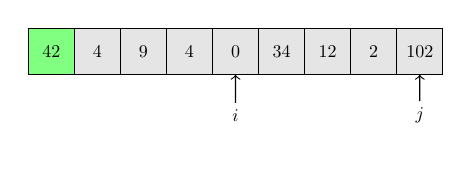
\begin{tikzpicture}[scale=.65,transform shape]

\def\sz{9mm}
\tikzstyle{block} = [
	draw, fill=black!10, rectangle,
	minimum height=\sz, minimum width=\sz ];
\tikzstyle{plain} = [draw=none,fill=none];
\draw[white] (0,0) rectangle (1, -2.15);

\node[block,fill=green!50] (a0) at (0*\sz,0) { 42 };
\node[block] (a1) at (1*\sz,0) { 4 };
\node[block] (a2) at (2*\sz,0) { 9 };
\node[block] (a3) at (3*\sz,0) { 4 };
\node[block] (a4) at (4*\sz,0) { 0 };
\node[block] (a5) at (5*\sz,0) { 34 };
\node[block] (a6) at (6*\sz,0) { 12 };
\node[block] (a7) at (7*\sz,0) { 2 };
\node[block] (a8) at (8*\sz,0) { 102 };

\node[below of=a4,node distance=1.25cm] (c4) {$i$};
\draw[->] (c4) -- (a4);
\node[below of=a8,node distance=1.25cm] (d1) {$j$};
\draw[->] (d1) -- (a8);

\end{tikzpicture}

}

\subfigure[Second iteration.  The index variable $i$ moves all the way to the
right as all remaining elements are less than the pivot, 42.  The index
variable $j$ remains at 102 as $i$ is now equal to $j$.]{

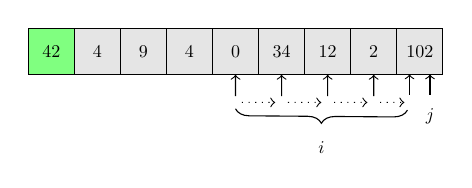
\begin{tikzpicture}[scale=.65,transform shape]

%\tikzset{>=stealth',shorten <=.2cm,>=stealth',shorten >=.2cm}
% size of each node
\def\sz{9mm}
% node style definition
\tikzstyle{block} = [
	draw, fill=black!10, rectangle,
	minimum height=\sz, minimum width=\sz ];
\tikzstyle{plain} = [draw=none,fill=none];

%\node[plain] at (-1.75, 1) { index };
%\node[plain] at (0*\sz,1.0) { 0 };
%\node[plain] at (1*\sz,1.0) { 1 };
%\node[plain] at (2*\sz,1.0) { 2 };
%\node[plain] at (3*\sz,1.0) { 3 };
%\node[plain] at (4*\sz,1.0) { 4 };
%\node[plain] at (5*\sz,1.0) { 5 };
%\node[plain] at (6*\sz,1.0) { 6 };
%\node[plain] at (7*\sz,1.0) { 7 };
%\node[plain] at (8*\sz,1.0) { 8 };
%\node[plain] at (-1.75, 0) { contents };
%

\node[block,fill=green!50] (a0) at (0*\sz,0) { 42 };
\node[block] (a1) at (1*\sz,0) { 4 };
\node[block] (a2) at (2*\sz,0) { 9 };
\node[block] (a3) at (3*\sz,0) { 4 };
\node[block] (a4) at (4*\sz,0) { 0 };
\node[block] (a5) at (5*\sz,0) { 34 };
\node[block] (a6) at (6*\sz,0) { 12 };
\node[block] (a7) at (7*\sz,0) { 2 };
\node[block] (a8) at (8*\sz,0) { 102 };

\node[below of=a4] (c4) {};
\node[below of=a5] (c5) {};
\node[below of=a6] (c6) {};
\node[below of=a7] (c7) {};
%\node[below of=a8,xshift=-10pt] (c8) {};
\draw[->] (c4) -- (a4);
\draw[->] (c5) -- (a5);
\draw[->] (c6) -- (a6);
\draw[->] (c7) -- (a7);

\draw[->,dotted] (c4) -- (c5);
\draw[->,dotted] (c5) -- (c6);
\draw[->,dotted] (c6) -- (c7);
\draw[->,dotted] (c7) -- (6.9,-1.0);

\node[below of=a8] (d1) {~};
\draw[->] (7.4,-0.85) -- (7.4,-0.45);
\draw[->] (7.0,-0.85) -- (7.0,-0.45);
\node[below] at (7.4, -1) {$j$};

\draw [decorate,decoration={brace,mirror,amplitude=5pt},xshift=-4pt,yshift=0pt] ([xshift=0cm,yshift=0cm]c4.south) -- (7.1,-1.15) node [black,midway,yshift=-0.75cm] {$i$};

%\draw[<->,>=stealth',shorten <=.2cm,>=stealth',shorten >=.2cm] (a4.south) to [bend right] node[pos=.5,below] {swap} (a8.south);

%\draw[<->] (a4.south) to [in=270,out=270,looseness=1] node[pos=.5,below] {swap} (a8.south);

\end{tikzpicture}~~~~~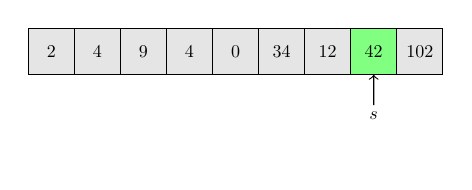
\begin{tikzpicture}[scale=.65,transform shape]

\def\sz{9mm}
\tikzstyle{block} = [
	draw, fill=black!10, rectangle,
	minimum height=\sz, minimum width=\sz ];
\tikzstyle{plain} = [draw=none,fill=none];
\draw[white] (0,0) rectangle (1, -2.15);

\node[block] (a0) at (0*\sz,0) { 2 };
\node[block] (a1) at (1*\sz,0) { 4 };
\node[block] (a2) at (2*\sz,0) { 9 };
\node[block] (a3) at (3*\sz,0) { 4 };
\node[block] (a4) at (4*\sz,0) { 0 };
\node[block] (a5) at (5*\sz,0) { 34 };
\node[block] (a6) at (6*\sz,0) { 12 };
\node[block,fill=green!50] (a7) at (7*\sz,0) { 42 };
\node[block] (a8) at (8*\sz,0) { 102 };

%\node[below of=a4,node distance=1.25cm] (c4) {$i$};
%\draw[->] (c4) -- (a4);
\node[below of=a7,node distance=1.25cm] (d1) {$s$};
\draw[->] (d1) -- (a7);

\end{tikzpicture}

}

\caption[Partitioning Example 1]{Example execution of the \textsc{Partition}
subroutine in Quick Sort.  A total of 8 comparisons are made, 9 if you count
the last swap outside the while loop.  The partition returns $s$ as the
pivot position; the right-partition is sorted as it only consists of 1 element.}
\label{figure:partitionExample1}

\end{figure}


%\end{document}


%\documentclass[12pt]{scrbook}
%
%\usepackage{tikz}
%\usepackage{minted}
%\usetikzlibrary{decorations.pathreplacing,arrows}
%\usetikzlibrary{arrows,decorations.pathmorphing,backgrounds,positioning,fit,petri}
%
%\usepackage{fullpage}
%\usepackage{subfigure}
%\begin{document}
%
%
%Lorem Ipsum is simply dummy text of the printing and typesetting industry. Lorem Ipsum has been the industry's standard dummy text ever since the 1500s, when an unknown printer took a galley of type and scrambled it to make a type specimen book. It has survived not only five centuries, but also the leap into electronic typesetting, remaining essentially unchanged. It was popularised in the 1960s with the release of Letraset sheets containing Lorem Ipsum passages, and more recently with desktop publishing software like Aldus PageMaker including versions of Lorem Ipsum.





\begin{figure}
\centering

\subfigure[First iteration.  In this partitioning, 2 is the pivot element.
The index variable $i$ is not incremented as 4 is larger than the pivot.
The index variable $j$ decrements to 0 and they are swapped.]{

\begin{tikzpicture}[scale=.65,transform shape]

%\tikzset{>=stealth',shorten <=.2cm,>=stealth',shorten >=.2cm}
% size of each node
\def\sz{9mm}
% node style definition
\tikzstyle{block} = [
	draw, fill=black!10, rectangle,
	minimum height=\sz, minimum width=\sz ];
\tikzstyle{plain} = [draw=none,fill=none];

\node[block,fill=green!50] (a0) at (0*\sz,0) { 2 };
\node[block] (a1) at (1*\sz,0) { 4 };
\node[block] (a2) at (2*\sz,0) { 9 };
\node[block] (a3) at (3*\sz,0) { 4 };
\node[block] (a4) at (4*\sz,0) { 0 };
\node[block] (a5) at (5*\sz,0) { 34 };
\node[block] (a6) at (6*\sz,0) { 12 };

\node[below of=a1] (c1) {};
\draw[->] (c1) -- (a1);

\node[below of=a4] (d4) {};
\draw[->] (d4) -- (a4);
\node[below of=a5] (d5) {};
\draw[->] (d5) -- (a5);
\node[below of=a6] (d6) {};
\draw[->] (d6) -- (a6);
\draw[<-,dotted] (d4) -- (d5);
\draw[<-,dotted] (d5) -- (d6);
\node[below of=d4,above] {$j$};
\node[below of=c1,above] {$i$};

%\draw [decorate,decoration={brace,mirror,amplitude=5pt},xshift=-4pt,yshift=0pt] ([xshift=0cm,yshift=0cm]c1.south) -- ([xshift=0cm,yshift=0cm]c4.south) node [black,midway,yshift=-0.75cm] {$i$};

\draw[<->,>=stealth',shorten <=.2cm,>=stealth',shorten >=.2cm] (a1.south) to [bend right] node[pos=.5,below] {swap} (a4.south);

%\draw[<->] (a4.south) to [in=270,out=270,looseness=1] node[pos=.5,below] {swap} (a8.south);

\end{tikzpicture}~~~~~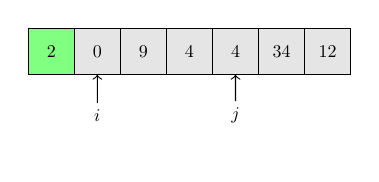
\begin{tikzpicture}[scale=.65,transform shape]

\def\sz{9mm}
\tikzstyle{block} = [
	draw, fill=black!10, rectangle,
	minimum height=\sz, minimum width=\sz ];
\tikzstyle{plain} = [draw=none,fill=none];
\draw[white] (0,0) rectangle (1, -2);

\node[block,fill=green!50] (a0) at (0*\sz,0) { 2 };
\node[block] (a1) at (1*\sz,0) { 0 };
\node[block] (a2) at (2*\sz,0) { 9 };
\node[block] (a3) at (3*\sz,0) { 4 };
\node[block] (a4) at (4*\sz,0) { 4 };
\node[block] (a5) at (5*\sz,0) { 34 };
\node[block] (a6) at (6*\sz,0) { 12 };

\node[below of=a1,node distance=1.25cm] (c4) {$i$};
\draw[->] (c4) -- (a1);
\node[below of=a4,node distance=1.25cm] (d1) {$j$};
\draw[->] (d1) -- (a4);

\end{tikzpicture}

}

\subfigure[Second iteration.  The index variable $i$ is incremented
once, while $j$ is decremented to meet it.  After the while loop the
second case applies as $a_i = 9 > 2 = pivot$, and so we swap 
$a_{i-1} = 2$ with the pivot.]{

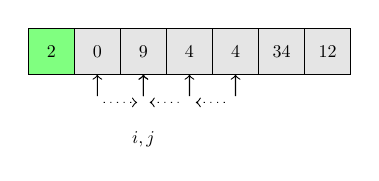
\begin{tikzpicture}[scale=.65,transform shape]

%\tikzset{>=stealth',shorten <=.2cm,>=stealth',shorten >=.2cm}
% size of each node
\def\sz{9mm}
% node style definition
\tikzstyle{block} = [
	draw, fill=black!10, rectangle,
	minimum height=\sz, minimum width=\sz ];
\tikzstyle{plain} = [draw=none,fill=none];

\node[block,fill=green!50] (a0) at (0*\sz,0) { 2 };
\node[block] (a1) at (1*\sz,0) { 0 };
\node[block] (a2) at (2*\sz,0) { 9 };
\node[block] (a3) at (3*\sz,0) { 4 };
\node[block] (a4) at (4*\sz,0) { 4 };
\node[block] (a5) at (5*\sz,0) { 34 };
\node[block] (a6) at (6*\sz,0) { 12 };

\node[below of=a1] (c1) {};
\draw[->] (c1) -- (a1);
\node[below of=a2] (c2) {};
\draw[->] (c2) -- (a2);
\draw[->,dotted] (c1) -- (c2);

\node[below of=a2] (d2) {};
\draw[->] (d2) -- (a2);
\node[below of=a3] (d3) {};
\draw[->] (d3) -- (a3);
\node[below of=a4] (d4) {};
\draw[->] (d4) -- (a4);
\draw[<-,dotted] (d3) -- (d4);
\draw[<-,dotted] (d2) -- (d3);
\node[below of=c2,above] {$i,j$};


%\draw[<->,>=stealth',shorten <=.2cm,>=stealth',shorten >=.2cm] (a1.south) to [bend right] node[pos=.5,below] {swap} (a4.south);

\end{tikzpicture}~~~~~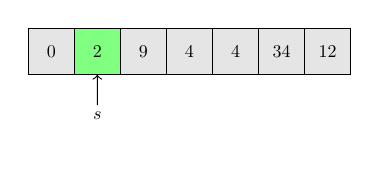
\begin{tikzpicture}[scale=.65,transform shape]

\def\sz{9mm}
\tikzstyle{block} = [
	draw, fill=black!10, rectangle,
	minimum height=\sz, minimum width=\sz ];
\tikzstyle{plain} = [draw=none,fill=none];
\draw[white] (0,0) rectangle (1, -2);

\node[block] (a0) at (0*\sz,0) { 0 };
\node[block,fill=green!50] (a1) at (1*\sz,0) { 2 };
\node[block] (a2) at (2*\sz,0) { 9 };
\node[block] (a3) at (3*\sz,0) { 4 };
\node[block] (a4) at (4*\sz,0) { 4 };
\node[block] (a5) at (5*\sz,0) { 34 };
\node[block] (a6) at (6*\sz,0) { 12 };

\node[below of=a1,node distance=1.25cm] (c4) {$s$};
\draw[->] (c4) -- (a1);

\end{tikzpicture}

}

\caption[Partitioning Example 2]{Example execution of the \textsc{Partition}
subroutine in Quick Sort on the first recursive call on the left partition.  
A total of 6 comparisons are made, 7 if you count the last swap outside the 
while loop.  The partition returns $s$ as the pivot position; in this case
the left-partition is sorted as it only consists of 1 element.}
\label{figure:partitionExample2}

\end{figure}


%\end{document}


%\documentclass[12pt]{scrbook}
%
%\usepackage{tikz}
%\usepackage{minted}
%\usetikzlibrary{decorations.pathreplacing,arrows}
%\usetikzlibrary{arrows,decorations.pathmorphing,backgrounds,positioning,fit,petri}
%
%\usepackage{fullpage}
%\usepackage{subfigure}
%\begin{document}
%
%
%Lorem Ipsum is simply dummy text of the printing and typesetting industry. Lorem Ipsum has been the industry's standard dummy text ever since the 1500s, when an unknown printer took a galley of type and scrambled it to make a type specimen book. It has survived not only five centuries, but also the leap into electronic typesetting, remaining essentially unchanged. It was popularised in the 1960s with the release of Letraset sheets containing Lorem Ipsum passages, and more recently with desktop publishing software like Aldus PageMaker including versions of Lorem Ipsum.
%




\begin{figure}
\centering

\subfigure[First (and only) iteration.  In this partitioning, 9 is the pivot.
The index variable $i$ is incremented to 34 while $j$ decrements 
to match.  34 is swapped with itself.  After this iteration, the second
condition applies and the pivot is swapped with $a_{i-1} = 4$]{

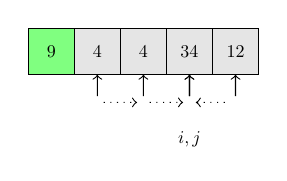
\begin{tikzpicture}[scale=.65,transform shape]

%\tikzset{>=stealth',shorten <=.2cm,>=stealth',shorten >=.2cm}
% size of each node
\def\sz{9mm}
% node style definition
\tikzstyle{block} = [
	draw, fill=black!10, rectangle,
	minimum height=\sz, minimum width=\sz ];
\tikzstyle{plain} = [draw=none,fill=none];

\node[block,fill=green!50] (a0) at (0*\sz,0) { 9 };
\node[block] (a1) at (1*\sz,0) { 4 };
\node[block] (a2) at (2*\sz,0) { 4 };
\node[block] (a3) at (3*\sz,0) { 34 };
\node[block] (a4) at (4*\sz,0) { 12 };

\node[below of=a1] (c1) {};
\draw[->] (c1) -- (a1);
\node[below of=a2] (c2) {};
\draw[->] (c2) -- (a2);
\node[below of=a3] (c3) {};
\draw[->] (c3) -- (a3);
\draw[->,dotted] (c1) -- (c2);
\draw[->,dotted] (c2) -- (c3);

\node[below of=a3] (d3) {};
\draw[->] (d3) -- (a3);
\node[below of=a4] (d4) {};
\draw[->] (d4) -- (a4);

\draw[<-,dotted] (d3) -- (d4);
\node[below of=c3,above] {$i,j$};


%\draw [decorate,decoration={brace,mirror,amplitude=5pt},xshift=-4pt,yshift=0pt] ([xshift=0cm,yshift=0cm]c1.south) -- ([xshift=0cm,yshift=0cm]c4.south) node [black,midway,yshift=-0.75cm] {$i$};

%\draw[<->,>=stealth',shorten <=.2cm,>=stealth',shorten >=.2cm] (a1.south) to [bend right] node[pos=.5,below] {swap} (a4.south);

%\draw[<->] (a4.south) to [in=270,out=270,looseness=1] node[pos=.5,below] {swap} (a8.south);

\end{tikzpicture}~~~~~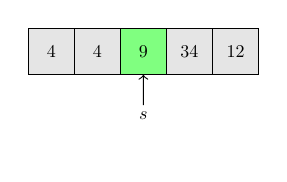
\begin{tikzpicture}[scale=.65,transform shape]

\def\sz{9mm}
\tikzstyle{block} = [
	draw, fill=black!10, rectangle,
	minimum height=\sz, minimum width=\sz ];
\tikzstyle{plain} = [draw=none,fill=none];
\draw[white] (0,0) rectangle (1, -2);

\node[block] (a0) at (0*\sz,0) { 4 };
\node[block] (a1) at (1*\sz,0) { 4 };
\node[block,fill=green!50] (a2) at (2*\sz,0) { 9 };
\node[block] (a3) at (3*\sz,0) { 34 };
\node[block] (a4) at (4*\sz,0) { 12 };

\node[below of=a2,node distance=1.25cm] (c2) {$s$};
\draw[->] (c2) -- (a2);

\end{tikzpicture}

}

\caption[Partitioning Example 3]{Example execution of the \textsc{Partition}
subroutine in Quick Sort on the second recursive call on the right partition.  
A total of 5 comparisons are made, 6 if you count the last swap outside the 
while loop.  The partition returns $s$ as the pivot position.}
\label{figure:partitionExample3}

\end{figure}


%\end{document}



\subsubsection{Analysis}

We can easily analyze how many comparisons are made by the \textsc{Partition}
subroutine.  Suppose that we are given a (sub)array of $n$ elements.  Since 
the pivot element must be compared to every other element in the (sub)array, 
it must make $n-1$ comparisons to partition the elements around the pivot.
If we count the last comparison to determine where to place the pivot, it 
would be $n$ comparisons (but the difference is trivial).  

The analysis of Quick Sort itself is a bit more involved and is highly
dependent on how well the \textsc{Partition} subroutine splits the
array.  In the worst case, our pivot choice will always partition the
array into one ``empty'' subarray and one subarray with $n-1$ elements
(we do not count the pivot element).  One such example of this would
be if our collection is already sorted.  In this case, one of the
recursive calls would result in no comparisons and the other would result
in $n-1$ comparisons.  This lopsided recursion would result in the
following number of comparisons:
$$n + (n-1) + (n-2) + \cdots + 3 + 2 + 1$$
which is exactly Gauss's Formula, meaning that Quick Sort would perform
$$\frac{n(n+1)}{2}$$
in the worst case.

However, in the sorting scenario, we cannot always assume the worst case.
If we are given random data, then the likelihood that we will always have
such an extremely lopsided partitioning is extremely small.  A more reasonable
analysis would involve the average case: where each partition is roughly an
equal size, \emph{about} $\frac{n}{2}$.  This happens when our pivot
choice is the median (or \emph{close} to the median) element.

To analyze the number of comparisons in this case, we can setup a 
\emph{recurrence relation}:
  $$C(n) = 2C\left( \frac{n}{2} \right) + n$$
Here, $C(n)$ represents the number of comparisons made by Quick Sort
on an array of size $n$.  The first term on the right hand side represents
the fact that we make 2 recursive calls on subarrays of size (roughly)
$\frac{n}{2}$.  The second term captures the number of comparisons we
make in the \textsc{Partition} subroutine.  Solving this recurrence is
a bit beyond the scope of the current discussion.  However, it can be
shown that this is roughly equivalent to 
  $$n\log{(n)}$$
comparisons in the best case.  

The difference between the best and worst case scenarios is in our pivot
choice.  Though the ideal pivot choice is the median element,
to find the median the usual strategy is to sort the collection first. 
This puts the cart before the horse.  If the data we are sorting is
in more-or-less random order, then the choice of the first element as a
pivot is good enough as it is unlikely that we will always have a 
bad paritioning.  However, there are other strategies.

One strategy is to randomly choose a pivot element.  A random choice 
would make the worst-case scenario very unlikely over many runs of the
algorithm.  Another strategy is to choose the median of three elements 
(either fixed or randomized), ensuring that neither partition will ever
be empty.  This strategy can be taken further to find the 
median-of-three amongst each third of the array and then take the median
of these (or the ``ninther'').  The more effort you put into finding the
median the more the performance degrades in practice.\footnote{For
example, there does exist a median-finding algorithm that runs in
linear time which would guarantee the theoretically best running time, but
the algorithm is recursive and has a large overhead, making its use
slow in practice.}  A more sophisticated analysis of these strategies
yields a complexity similar to the best case \cite{Bentley:1993:ESF:172704.172710}.

\subsection{Merge Sort}
\index{Merge Sort}
\index{sorting!Merge Sort}

Another ``fast'' sorting algorithm is Merge Sort, due to John von 
Neumann, 1945 (as reported by Knuth \cite{Knuth:1970:VNF:356580.356581}).
The performance is similar to Quick Sort's best/average case, making
  $$n \log{(n)}$$
comparisons.  However, Merge Sort's performance does not depend on the
structure of the input array or a pivot choice, guaranteeing this performance
in the best/average/worst case.\footnote{Still, Quick Sort is still more common
in practice because it has less memory requirements and the pivot choice
strategies can mitigate the risk of the worst-case scenario.}

Merge Sort works by \emph{first} dividing the list into two (roughly) 
equal partitions.  It then recursively sorts each partition.  The
recursion stops when the subarray is of size $\leq 1$ just as with Quick
Sort.  The difference, however, is what Merge Sort does after the
recursion.  After having sorted the left partition, $L$ and the right
partition $R$, Merge Sort \emph{merges} the two sorted partitions into
one.

The \textsc{Merge} subroutine works by maintaining two index variables, 
$i, j$, one for each partition.  Suppose that the index variables 
correspond to the elements $L_i$ and $R_j$ in the left/right partition.
If $L_i \leq R_j$, we add $L_i$ to the end of a temporary array and
increment $i$.  Otherwise we place $R_j$ into the temporary array
and increment $j$.  We continue until we have examined every element
in one or both partitions (if one partition still has elements in it, 
we can simply copy the rest over in order).  This merge operation works
because each subarray is sorted.

Merge Sort is presented as Algorithm \ref{algo:mergeSort} with the
\textsc{Merge} subroutine as Algorithm \ref{algo:merge}.

\begin{algorithm}
  \Input{A (sub)collection $A = \{a_l, \ldots, a_r\}$, indices $l, r$}
  \Output{A collection $A'$ which is $A$ sorted}
  \eIf{$l < r$} {
    $m \leftarrow \lfloor\frac{l+r}{2}\rfloor$ \;
    $L \leftarrow \textsc{MergeSort}(A, l, m)$ \;
    $R \leftarrow \textsc{MergeSort}(A, m+1, r)$ \;
    output $\textsc{Merge}(L, R)$ \;    
  }{
    output $A$ \;
  }
\caption{\textsc{MergeSort}}
\label{algo:mergeSort}
\end{algorithm}

\begin{algorithm}[H]
  \Input{Two sorted collections, $L$, $R$ of size $n, m$ respectively.}
  \Output{A sorted collection $A$ consisting of all elements of $L$ and $R$}
  $A \leftarrow $ a new, empty collection \;
  $i \leftarrow 1$ \;
  $j \leftarrow 1$ \;
  $k \leftarrow 1$ \Comment{index variable for $A$} \;
  \While{$i \leq n \And j \leq m$}{
    \eIf{$L_i \leq R_i$}{
      $A_k \leftarrow L_i$ \;
      $i \leftarrow (i+1)$ \;
    }{
      $A_k \leftarrow L_j$ \;
      $j \leftarrow (j+1)$ \;
    }
    $k \leftarrow (k+1)$ \;
  }
  \Comment{At least one collection is empty, we can blindly copy the other}
  \While{$i \leq n$}{
    $A_k \leftarrow L_i$ \;
    $i \leftarrow (i+1)$ \;
    $k \leftarrow (k+1)$ \;
  }
  \While{$j \leq m$}{
    $A_k \leftarrow R_j$ \;
    $j \leftarrow (j+1)$ \;
    $k \leftarrow (k+1)$ \;
  }
  output $A$ \;
\caption{\textsc{Merge}}
\label{algo:merge}
\end{algorithm}

We present an example run of Merge Sort in Figure \ref{figure:mergeSortExample}
(here, we have made the collection of size 8 to emphasize the even split).  
An example run of the \textsc{Merge} subroutine on the last merge operation
of this algorithm is presented in Figure \ref{figure:mergeExample}.

%\documentclass[12pt]{scrbook}
%
%\usepackage{tikz}
%\usepackage{minted}
%%\usetikzlibrary{decorations.pathreplacing}
%%
%\usetikzlibrary{patterns}
%\usetikzlibrary{decorations.pathreplacing,arrows}
%\usetikzlibrary{arrows,decorations.pathmorphing,backgrounds,positioning,fit,petri}
%
%\usepackage{fullpage}
%\usepackage{subfigure}
%\begin{document}
%
%
%Lorem Ipsum is simply dummy text of the printing and typesetting industry. Lorem Ipsum has been the industry's standard dummy text ever since the 1500s, when an unknown printer took a galley of type and scrambled it to make a type specimen book. It has survived not only five centuries, but also the leap into electronic typesetting, remaining essentially unchanged. It was popularised in the 1960s with the release of Letraset sheets containing Lorem Ipsum passages, and more recently with desktop publishing software like Aldus PageMaker including versions of Lorem Ipsum.

\begin{figure}
\centering

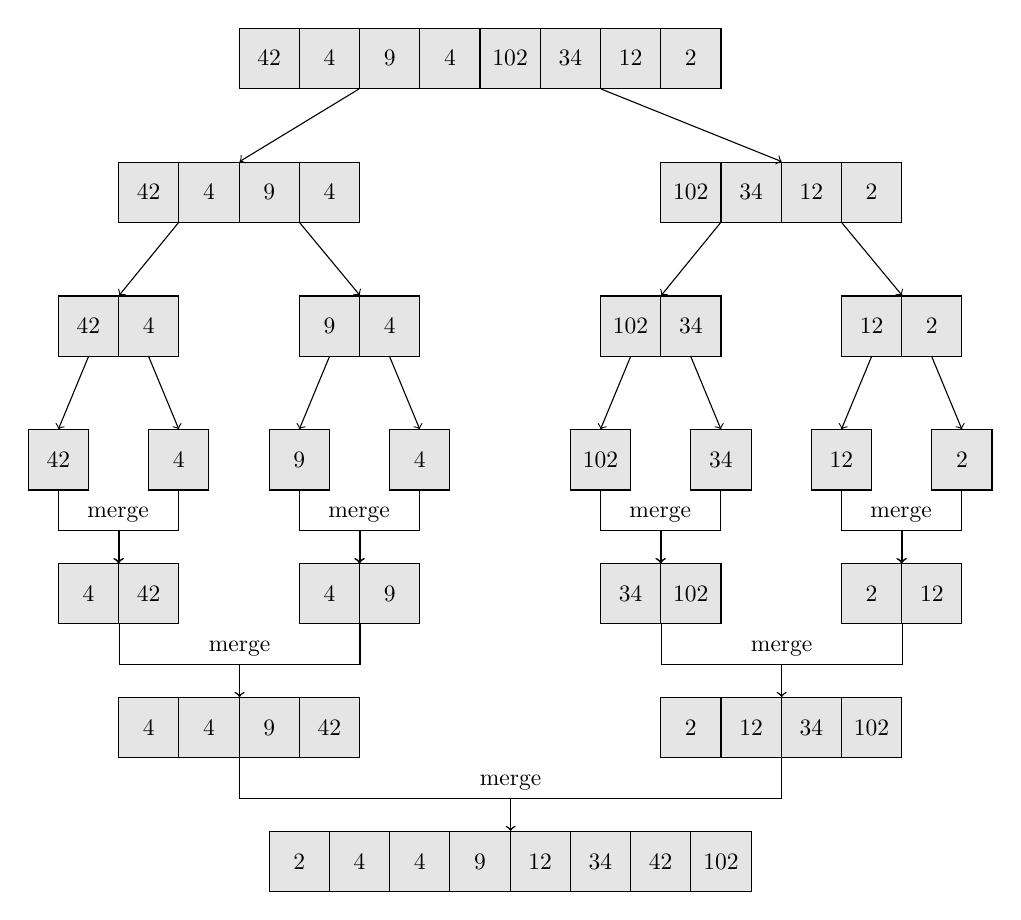
\begin{tikzpicture}[scale=.85,transform shape]

%\tikzset{>=stealth',shorten <=.2cm,>=stealth',shorten >=.2cm}
% size of each node
\def\sz{9mm}
% node style definition
\tikzstyle{block} = [
	draw, fill=black!10, rectangle,
	minimum height=\sz, minimum width=\sz ];
\tikzstyle{plain} = [draw=none,fill=none];

\node[block] (a0) at (0*\sz,0) { 42 };
\node[block] (a1) at (1*\sz,0) { 4 };
\node[block] (a2) at (2*\sz,0) { 9 };
\node[block] (a3) at (3*\sz,0) { 4 };
\node[block] (a4) at (4*\sz,0) { 102 };
\node[block] (a5) at (5*\sz,0) { 34 };
\node[block] (a6) at (6*\sz,0) { 12 };
\node[block] (a7) at (7*\sz,0) { 2 };

\node[block] (aa0) at (-2*\sz,-2) { 42 };
\node[block] (aa1) at (-1*\sz,-2) { 4 };
\node[block] (aa2) at (0*\sz,-2) { 9 };
\node[block] (aa3) at (1*\sz,-2) { 4 };

\node[block] (aa4) at (7*\sz,-2) { 102 };
\node[block] (aa5) at (8*\sz,-2) { 34 };
\node[block] (aa6) at (9*\sz,-2) { 12 };
\node[block] (aa7) at (10*\sz,-2) { 2 };

\node[block] (aaa0) at (-3*\sz,-4) { 42 };
\node[block] (aaa1) at (-2*\sz,-4) { 4 };

\node[block] (aaa2) at (1*\sz,-4) { 9 };
\node[block] (aaa3) at (2*\sz,-4) { 4 };

\node[block] (aaa4) at (6*\sz,-4) { 102 };
\node[block] (aaa5) at (7*\sz,-4) { 34 };

\node[block] (aaa6) at (10*\sz,-4) { 12 };
\node[block] (aaa7) at (11*\sz,-4) { 2 };

\node[block] (aaaa0) at (-3.5*\sz,-6) { 42 };
\node[block] (aaaa1) at (-1.5*\sz,-6) { 4 };
\node[block] (aaaa2) at (0.5*\sz,-6) { 9 };
\node[block] (aaaa3) at (2.5*\sz,-6) { 4 };

\node[block] (aaaa4) at (5.5*\sz,-6) { 102 };
\node[block] (aaaa5) at (7.5*\sz,-6) { 34 };
\node[block] (aaaa6) at (9.5*\sz,-6) { 12 };
\node[block] (aaaa7) at (11.5*\sz,-6) { 2 };

\draw[->] (a2.south west) -- (aa1.north east);
\draw[->] (a5.south east) -- (aa5.north east);

\draw[->] (aa1.south west) -- (aaa0.north east);
\draw[->] (aa2.south east) -- (aaa2.north east);
\draw[->] (aa5.south west) -- (aaa4.north east);
\draw[->] (aa6.south east) -- (aaa6.north east);

\draw[->] (aaa0.south) -- (aaaa0.north);
\draw[->] (aaa1.south) -- (aaaa1.north);
\draw[->] (aaa2.south) -- (aaaa2.north);
\draw[->] (aaa3.south) -- (aaaa3.north);
\draw[->] (aaa4.south) -- (aaaa4.north);
\draw[->] (aaa5.south) -- (aaaa5.north);
\draw[->] (aaa6.south) -- (aaaa6.north);
\draw[->] (aaa7.south) -- (aaaa7.north);

\node[block] (bbb0) at (-3*\sz,-8) { 4 };
\node[block] (bbb1) at (-2*\sz,-8) { 42 };

\node[block] (bbb2) at (1*\sz,-8) { 4 };
\node[block] (bbb3) at (2*\sz,-8) { 9 };

\node[block] (bbb4) at (6*\sz,-8) { 34 };
\node[block] (bbb5) at (7*\sz,-8) { 102 };

\node[block] (bbb6) at (10*\sz,-8) { 2 };
\node[block] (bbb7) at (11*\sz,-8) { 12 };

\node[block] (bb0) at (-2*\sz,-10) { 4 };
\node[block] (bb1) at (-1*\sz,-10) { 4 };
\node[block] (bb2) at (0*\sz,-10) { 9 };
\node[block] (bb3) at (1*\sz,-10) { 42 };

\node[block] (bb4) at (7*\sz,-10) { 2 };
\node[block] (bb5) at (8*\sz,-10) { 12 };
\node[block] (bb6) at (9*\sz,-10) { 34 };
\node[block] (bb7) at (10*\sz,-10) { 102 };

\node[block] (b0) at (0.5*\sz,-12) { 2 };
\node[block] (b1) at (1.5*\sz,-12) { 4 };
\node[block] (b2) at (2.5*\sz,-12) { 4 };
\node[block] (b3) at (3.5*\sz,-12) { 9 };
\node[block] (b4) at (4.5*\sz,-12) { 12 };
\node[block] (b5) at (5.5*\sz,-12) { 34 };
\node[block] (b6) at (6.5*\sz,-12) { 42 };
\node[block] (b7) at (7.5*\sz,-12) { 102 };

\draw[->] (aaaa0.south) -- ++(0,-0.6) -| (bbb0.north east);
\draw[->] (aaaa1.south) -- ++(0,-0.6) -| node[above] {merge} (bbb1.north west);
\draw[->] (aaaa2.south) -- ++(0,-0.6) -| (bbb2.north east);
\draw[->] (aaaa3.south) -- ++(0,-0.6) -| node[above] {merge} (bbb3.north west);
\draw[->] (aaaa4.south) -- ++(0,-0.6) -| (bbb4.north east);
\draw[->] (aaaa5.south) -- ++(0,-0.6) -| node[above] {merge} (bbb5.north west);
\draw[->] (aaaa6.south) -- ++(0,-0.6) -| (bbb6.north east);
\draw[->] (aaaa7.south) -- ++(0,-0.6) -| node[above] {merge} (bbb7.north west);

\draw[->] (bbb0.south east) -- ++(0,-0.6) -| (bb1.north east);
\draw[->] (bbb2.south east) -- ++(0,-0.6) -| node[above] {merge} (bb1.north east);
\draw[->] (bbb4.south east) -- ++(0,-0.6) -| (bb5.north east);
\draw[->] (bbb6.south east) -- ++(0,-0.6) -| node[above] {merge} (bb5.north east);

\draw[->] (bb1.south east) -- ++(0,-0.6) -| (b3.north east);
\draw[->] (bb5.south east) -- ++(0,-0.6) -| node[above] {merge} (b3.north east);

\end{tikzpicture}

\caption[Merge Sort Example]{Illustration of Merge Sort's recursion and
merge operations.}
\label{figure:mergeSortExample}
\end{figure}

\begin{figure}
\centering

\subfigure[Iteration One.  $L_1 = 4 > R_1 = 2$, so the element
in the right partition is copied into $A_1$.  Both $j, k$ are
incremented.]{

\begin{tikzpicture}[scale=.75,transform shape]

%\tikzset{>=stealth',shorten <=.2cm,>=stealth',shorten >=.2cm}
% size of each node
\def\sz{9mm}
% node style definition
\tikzstyle{block} = [
	draw, fill=black!10, rectangle,
	minimum height=\sz, minimum width=\sz ];
\tikzstyle{plain} = [draw=none,fill=none];

\node[block] (b0) at (0*\sz,0) { 4 };
\node[block] (b1) at (1*\sz,0) { 4 };
\node[block] (b2) at (2*\sz,0) { 9 };
\node[block] (b3) at (3*\sz,0) { 42 };

\node[block,fill=green!50] (b4) at (5*\sz,0) { 2 };
\node[block] (b5) at (6*\sz,0) { 12 };
\node[block] (b6) at (7*\sz,0) { 34 };
\node[block] (b7) at (8*\sz,0) { 102 };

\node[below of=b0] (i) {$i$};
\node[below of=b4] (j) {$j$};

\draw[->] (i) -- (b0);
\draw[->] (j) -- (b4);

\node[block] (a0) at (0*\sz,-2.5) { 2 };
\node[block] (a1) at (1*\sz,-2.5) {  };
\node[block] (a2) at (2*\sz,-2.5) {  };
\node[block] (a3) at (3*\sz,-2.5) {  };
\node[block] (a4) at (4*\sz,-2.5) {  };
\node[block] (a5) at (5*\sz,-2.5) {  };
\node[block] (a6) at (6*\sz,-2.5) {  };
\node[block] (a7) at (7*\sz,-2.5) {  };

\node[below of=a0] (k) {$k$};
\draw[->] (k) -- (a0);

\draw[->] (j.south) -- ++(0,-0.25) -| (a0.north);

\end{tikzpicture}
}~~~~~\subfigure[Iteration Two.  Now the element in the left
partition is lesser and is copied, incrementing $i, k$]{

\begin{tikzpicture}[scale=.75,transform shape]

%\tikzset{>=stealth',shorten <=.2cm,>=stealth',shorten >=.2cm}
% size of each node
\def\sz{9mm}
% node style definition
\tikzstyle{block} = [
	draw, fill=black!10, rectangle,
	minimum height=\sz, minimum width=\sz ];
\tikzstyle{plain} = [draw=none,fill=none];

\node[block,fill=green!50] (b0) at (0*\sz,0) { 4 };
\node[block] (b1) at (1*\sz,0) { 4 };
\node[block] (b2) at (2*\sz,0) { 9 };
\node[block] (b3) at (3*\sz,0) { 42 };

\node[block,pattern=north west lines, pattern color=blue] (b4) at (5*\sz,0) { 2 };
\node[block] (b5) at (6*\sz,0) { 12 };
\node[block] (b6) at (7*\sz,0) { 34 };
\node[block] (b7) at (8*\sz,0) { 102 };

\node[below of=b0] (i) {$i$};
\node[below of=b5] (j) {$j$};

\draw[->] (i) -- (b0);
\draw[->] (j) -- (b5);

\node[block] (a0) at (0*\sz,-2.5) { 2 };
\node[block] (a1) at (1*\sz,-2.5) { 4 };
\node[block] (a2) at (2*\sz,-2.5) {  };
\node[block] (a3) at (3*\sz,-2.5) {  };
\node[block] (a4) at (4*\sz,-2.5) {  };
\node[block] (a5) at (5*\sz,-2.5) {  };
\node[block] (a6) at (6*\sz,-2.5) {  };
\node[block] (a7) at (7*\sz,-2.5) {  };

\node[below of=a1] (k) {$k$};
\draw[->] (k) -- (a1);

\draw[->] (i.south) -- ++(0,-0.25) -| (a1.north);

\end{tikzpicture}
}

\subfigure[Iteration Three.  Again the element in the
left partition is less.]{

\begin{tikzpicture}[scale=.75,transform shape]

%\tikzset{>=stealth',shorten <=.2cm,>=stealth',shorten >=.2cm}
% size of each node
\def\sz{9mm}
% node style definition
\tikzstyle{block} = [
	draw, fill=black!10, rectangle,
	minimum height=\sz, minimum width=\sz ];
\tikzstyle{plain} = [draw=none,fill=none];

\node[block,pattern=north west lines, pattern color=blue] (b0) at (0*\sz,0) { 4 };
\node[block,fill=green!50] (b1) at (1*\sz,0) { 4 };
\node[block] (b2) at (2*\sz,0) { 9 };
\node[block] (b3) at (3*\sz,0) { 42 };

\node[block,pattern=north west lines, pattern color=blue] (b4) at (5*\sz,0) { 2 };
\node[block] (b5) at (6*\sz,0) { 12 };
\node[block] (b6) at (7*\sz,0) { 34 };
\node[block] (b7) at (8*\sz,0) { 102 };

\node[below of=b1] (i) {$i$};
\node[below of=b5] (j) {$j$};

\draw[->] (i) -- (b1);
\draw[->] (j) -- (b5);

\node[block] (a0) at (0*\sz,-2.5) { 2 };
\node[block] (a1) at (1*\sz,-2.5) { 4 };
\node[block] (a2) at (2*\sz,-2.5) { 4 };
\node[block] (a3) at (3*\sz,-2.5) {  };
\node[block] (a4) at (4*\sz,-2.5) {  };
\node[block] (a5) at (5*\sz,-2.5) {  };
\node[block] (a6) at (6*\sz,-2.5) {  };
\node[block] (a7) at (7*\sz,-2.5) {  };

\node[below of=a2] (k) {$k$};
\draw[->] (k) -- (a2);

\draw[->] (i.south) -- ++(0,-0.25) -| (a2.north);

\end{tikzpicture}
}~~~~~\subfigure[Iteration Four.  And so on.]{

\begin{tikzpicture}[scale=.75,transform shape]

%\tikzset{>=stealth',shorten <=.2cm,>=stealth',shorten >=.2cm}
% size of each node
\def\sz{9mm}
% node style definition
\tikzstyle{block} = [
	draw, fill=black!10, rectangle,
	minimum height=\sz, minimum width=\sz ];
\tikzstyle{plain} = [draw=none,fill=none];

\node[block,pattern=north west lines, pattern color=blue] (b0) at (0*\sz,0) { 4 };
\node[block,pattern=north west lines, pattern color=blue] (b1) at (1*\sz,0) { 4 };
\node[block,fill=green!50] (b2) at (2*\sz,0) { 9 };
\node[block] (b3) at (3*\sz,0) { 42 };

\node[block,pattern=north west lines, pattern color=blue] (b4) at (5*\sz,0) { 2 };
\node[block] (b5) at (6*\sz,0) { 12 };
\node[block] (b6) at (7*\sz,0) { 34 };
\node[block] (b7) at (8*\sz,0) { 102 };

\node[below of=b2] (i) {$i$};
\node[below of=b5] (j) {$j$};

\draw[->] (i) -- (b2);
\draw[->] (j) -- (b5);

\node[block] (a0) at (0*\sz,-2.5) { 2 };
\node[block] (a1) at (1*\sz,-2.5) { 4 };
\node[block] (a2) at (2*\sz,-2.5) { 4};
\node[block] (a3) at (3*\sz,-2.5) { 9};
\node[block] (a4) at (4*\sz,-2.5) {  };
\node[block] (a5) at (5*\sz,-2.5) {  };
\node[block] (a6) at (6*\sz,-2.5) {  };
\node[block] (a7) at (7*\sz,-2.5) {  };

\node[below of=a3] (k) {$k$};
\draw[->] (k) -- (a3);

\draw[->] (i.south) -- ++(0,-0.25) -| (a3.north);

\end{tikzpicture}
}

\subfigure[Iteration Five]{

\begin{tikzpicture}[scale=.75,transform shape]

%\tikzset{>=stealth',shorten <=.2cm,>=stealth',shorten >=.2cm}
% size of each node
\def\sz{9mm}
% node style definition
\tikzstyle{block} = [
	draw, fill=black!10, rectangle,
	minimum height=\sz, minimum width=\sz ];
\tikzstyle{plain} = [draw=none,fill=none];

\node[block,pattern=north west lines, pattern color=blue] (b0) at (0*\sz,0) { 4 };
\node[block,pattern=north west lines, pattern color=blue] (b1) at (1*\sz,0) { 4 };
\node[block,pattern=north west lines, pattern color=blue] (b2) at (2*\sz,0) { 9 };
\node[block] (b3) at (3*\sz,0) { 42 };

\node[block,pattern=north west lines, pattern color=blue] (b4) at (5*\sz,0) { 2 };
\node[block,fill=green!50] (b5) at (6*\sz,0) { 12 };
\node[block] (b6) at (7*\sz,0) { 34 };
\node[block] (b7) at (8*\sz,0) { 102 };

\node[below of=b3] (i) {$i$};
\node[below of=b5] (j) {$j$};

\draw[->] (i) -- (b3);
\draw[->] (j) -- (b5);

\node[block] (a0) at (0*\sz,-2.5) { 2 };
\node[block] (a1) at (1*\sz,-2.5) { 4 };
\node[block] (a2) at (2*\sz,-2.5) { 4};
\node[block] (a3) at (3*\sz,-2.5) { 9};
\node[block] (a4) at (4*\sz,-2.5) { 12 };
\node[block] (a5) at (5*\sz,-2.5) {  };
\node[block] (a6) at (6*\sz,-2.5) {  };
\node[block] (a7) at (7*\sz,-2.5) {  };

\node[below of=a4] (k) {$k$};
\draw[->] (k) -- (a4);

\draw[->] (j.south) -- ++(0,-0.25) -| (a4.north);

\end{tikzpicture}
}~~~~~\subfigure[Iteration Six]{

\begin{tikzpicture}[scale=.75,transform shape]

%\tikzset{>=stealth',shorten <=.2cm,>=stealth',shorten >=.2cm}
% size of each node
\def\sz{9mm}
% node style definition
\tikzstyle{block} = [
	draw, fill=black!10, rectangle,
	minimum height=\sz, minimum width=\sz ];
\tikzstyle{plain} = [draw=none,fill=none];

\node[block,pattern=north west lines, pattern color=blue] (b0) at (0*\sz,0) { 4 };
\node[block,pattern=north west lines, pattern color=blue] (b1) at (1*\sz,0) { 4 };
\node[block,pattern=north west lines, pattern color=blue] (b2) at (2*\sz,0) { 9 };
\node[block] (b3) at (3*\sz,0) { 42 };

\node[block,pattern=north west lines, pattern color=blue] (b4) at (5*\sz,0) { 2 };
\node[block,pattern=north west lines, pattern color=blue] (b5) at (6*\sz,0) { 12 };
\node[block,fill=green!50] (b6) at (7*\sz,0) { 34 };
\node[block] (b7) at (8*\sz,0) { 102 };

\node[below of=b3] (i) {$i$};
\node[below of=b6] (j) {$j$};

\draw[->] (i) -- (b3);
\draw[->] (j) -- (b6);

\node[block] (a0) at (0*\sz,-2.5) { 2 };
\node[block] (a1) at (1*\sz,-2.5) { 4 };
\node[block] (a2) at (2*\sz,-2.5) { 4};
\node[block] (a3) at (3*\sz,-2.5) { 9};
\node[block] (a4) at (4*\sz,-2.5) { 12 };
\node[block] (a5) at (5*\sz,-2.5) { 34 };
\node[block] (a6) at (6*\sz,-2.5) {  };
\node[block] (a7) at (7*\sz,-2.5) {  };

\node[below of=a5] (k) {$k$};
\draw[->] (k) -- (a5);

\draw[->] (j.south) -- ++(0,-0.25) -| (a5.north);

\end{tikzpicture}
}

\subfigure[Iteration Seven]{

\begin{tikzpicture}[scale=.75,transform shape]

%\tikzset{>=stealth',shorten <=.2cm,>=stealth',shorten >=.2cm}
% size of each node
\def\sz{9mm}
% node style definition
\tikzstyle{block} = [
	draw, fill=black!10, rectangle,
	minimum height=\sz, minimum width=\sz ];
\tikzstyle{plain} = [draw=none,fill=none];

\node[block,pattern=north west lines, pattern color=blue] (b0) at (0*\sz,0) { 4 };
\node[block,pattern=north west lines, pattern color=blue] (b1) at (1*\sz,0) { 4 };
\node[block,pattern=north west lines, pattern color=blue] (b2) at (2*\sz,0) { 9 };
\node[block,fill=green!50] (b3) at (3*\sz,0) { 42 };

\node[block,pattern=north west lines, pattern color=blue] (b4) at (5*\sz,0) { 2 };
\node[block,pattern=north west lines, pattern color=blue] (b5) at (6*\sz,0) { 12 };
\node[block,pattern=north west lines, pattern color=blue] (b6) at (7*\sz,0) { 34 };
\node[block] (b7) at (8*\sz,0) { 102 };

\node[below of=b3] (i) {$i$};
\node[below of=b7] (j) {$j$};

\draw[->] (i) -- (b3);
\draw[->] (j) -- (b7);

\node[block] (a0) at (0*\sz,-2.5) { 2 };
\node[block] (a1) at (1*\sz,-2.5) { 4 };
\node[block] (a2) at (2*\sz,-2.5) { 4};
\node[block] (a3) at (3*\sz,-2.5) { 9};
\node[block] (a4) at (4*\sz,-2.5) { 12 };
\node[block] (a5) at (5*\sz,-2.5) { 34 };
\node[block] (a6) at (6*\sz,-2.5) { 42 };
\node[block] (a7) at (7*\sz,-2.5) {  };

\node[below of=a6] (k) {$k$};
\draw[->] (k) -- (a6);

\draw[->] (i.south) -- ++(0,-0.25) -| (a6.north);

\end{tikzpicture}
}~~~~~\subfigure[Final Copy.  After one sub-collection has been exhausted
the rest (in this case only one) of the elements in the other are blindly
copied over.]{

\begin{tikzpicture}[scale=.75,transform shape]

%\tikzset{>=stealth',shorten <=.2cm,>=stealth',shorten >=.2cm}
% size of each node
\def\sz{9mm}
% node style definition
\tikzstyle{block} = [
	draw, fill=black!10, rectangle,
	minimum height=\sz, minimum width=\sz ];
\tikzstyle{plain} = [draw=none,fill=none];

\node[block,pattern=north west lines, pattern color=blue] (b0) at (0*\sz,0) { 4 };
\node[block,pattern=north west lines, pattern color=blue] (b1) at (1*\sz,0) { 4 };
\node[block,pattern=north west lines, pattern color=blue] (b2) at (2*\sz,0) { 9 };
\node[block,pattern=north west lines, pattern color=blue] (b3) at (3*\sz,0) { 42 };

\node[block,pattern=north west lines, pattern color=blue] (b4) at (5*\sz,0) { 2 };
\node[block,pattern=north west lines, pattern color=blue] (b5) at (6*\sz,0) { 12 };
\node[block,pattern=north west lines, pattern color=blue] (b6) at (7*\sz,0) { 34 };
\node[block] (b7) at (8*\sz,0) { 102 };

\node[below of=b7] (j) {$j$};

\draw[->] (j) -- (b7);

\node[block] (a0) at (0*\sz,-2.5) { 2 };
\node[block] (a1) at (1*\sz,-2.5) { 4 };
\node[block] (a2) at (2*\sz,-2.5) { 4};
\node[block] (a3) at (3*\sz,-2.5) { 9};
\node[block] (a4) at (4*\sz,-2.5) { 12 };
\node[block] (a5) at (5*\sz,-2.5) { 34 };
\node[block] (a6) at (6*\sz,-2.5) { 42 };
\node[block] (a7) at (7*\sz,-2.5) { 102 };

\node[below of=a7] (k) {$k$};
\draw[->] (k) -- (a7);

\draw[->] (j.south) -- ++(0,-0.25) -| (a7.north);

\end{tikzpicture}
}
\caption[Merge Example]{Demonstration of the merge operation in Merge Sort.  Here
we depict the final \textsc{Merge} subroutine invocation from the previous
example.}
\label{figure:mergeExample}
\end{figure}



%\end{document}



\subsubsection{Analysis}

Because Merge Sort divides the list \emph{first}, an even split is
\emph{guaranteed}.  After the recursion, the \textsc{Merge} subroutine
requires at most $n-1$ comparisons to merge the two collections.  This
leads to a recurrence relation similar to Quick Sort, 
  $$C(n) = 2C\left( \frac{n}{2} \right) + (n-1)$$
A similar analysis yields a complexity of $n \log{(n)}$.

\subsection{Other Sorts}
\label{subsection:otherSorts}

There are dozens of other sorting algorithms and many more variations on
sorting algorithms, each with some unique properties and advantages.  
For example, Heap Sort, due to J.\ W.\ J.\ Williams, 1964 
\cite{williams1964algorithm}, uses a data structure called a \emph{heap}.
\index{Heap Sort}\index{sorting!Heap Sort}  A heap stores elements in
a \emph{tree} structure and offers efficient insertion of elements and
retrieval of the minimal (or maximal for a ``max-heap'') element.  The
sorting algorithm then simply inserts each element into the heap, and
retrieves each element out of the heap.  Because of the the heap data
structure, elements come out of the heap in order.  

Other sorting algorithms are variations on those we've already seen or
\emph{hybrid} sorting algorithms.  For example, we've already noted that
Insertion Sort is efficient on ``small'' arrays.  One common technique
is to use a fast sorting algorithm such as Quick Sort or Merge Sort, but
then switch over to Insertion Sort at some point in the recursion rather
than recursing to the point that the collection is of size 1 (or 0).  
This switch point is usually tuned using empirical experiments.  

A more recent sorting algorithm is Tim Sort, due to Tim Peters in 2002 
\cite{Peters2002} \index{Tim Sort}\index{sorting!Tim Sort} who originally 
developed it as the default sorting algorithm for the Python language.  
It has since been adopted in Java (version 7 for arrays of non-primitive 
types).  Tim Sort is a sort of ``bottom-up'' Merge Sort/Insertion Sort
hybrid.  Instead of recursing, it looks for subsequences of elements that
are already in order or nearly in order, then merges them.  It was designed
to have many of the desirable properties of a sorting algorithm 
including \emph{stability} (see Section \ref{subsection:sortingStability}).


\subsection{Comparison \& Summary}

To illustrate just how much more efficient an $n\log{(n)}$ sorting algorithm
is over a naive $n^2$ algorithm consider the same scenarios as with searching.
Suppose we want to sort a huge collection of 1 trillion, $10^{12}$, elements.
Doing so with Selection Sort or Insertion Sort would require about 
  $$n^2 = (10^{12})^2 = 10^{24}$$
or 1 septillion comparisons.  The same sorting operation using either
Quick Sort or Merge Sort would require only
  $$n\log{(n)} = 10^{12} \log{10^{12}} \approx 4 \times 10^{13}$$
or just under 40 trillion comparisons.  This is 25 \emph{billion} times
fewer operations.  

As another example, suppose that we sort a collection with $n$ elements
and then want to double the size of our collection to $2n$.  How do each
of these types of algorithms perform?  For the slow, $n^2$ algorithms we
have 
  $$(2n)^2 = 4n^2$$
Doubling the input size \emph{quadruples} the number of operations
Selection Sort and Insertion Sort perform.  However, for Quick Sort and
Merge Sort, we only have
  $$2n \log{(2n)} = 2n\left( \log{(2)} + \log{(n)}\right) = 2n\log{(n)} + 2n$$
That is, only about twice as many operations (with an additive term of $2n$). Table \ref{table:sortingSummary} gives a summary of the complexity and other
properties of the sorting algorithms we've seen.

\begin{table}[h]
\centering
\begin{tabular}{|c|c|c|c|c|p{4cm}|}
\hline
\multirow{2}{*}{Algorithm} & \multicolumn{3}{|c|}{Complexity} & \multirow{2}{*}{Stable?} & \multirow{2}{*}{Notes} \\ \cline{2-4}
~ & Best & Average & Worst & ~ & ~ \\
\hline
%Bubble Sort & $O(n^2)$ & $O(n^2)$ & $O(n^2)$ & Stable & \\
%\hline
Selection Sort & $\sim n^2$ & $\sim n^2$ & $\sim n^2$ & No & \\
\hline
Insertion Sort & $\sim n$ & $\sim n^2$ & $\sim n^2$ & Yes & Best in practice for small collections\\
\hline
Quick Sort & $\sim n\log{n}$ & $\sim n\log{n}$ & $\sim n^2$ & No & Performance depends on pivot choices\\
\hline
Merge Sort & $\sim n\log{n}$ & $\sim n\log{n}$ & $\sim n\log{n}$ & Yes & Requires extra space \\
\hline
\end{tabular}
\caption{Summary of Sorting Algorithms.  See Section
\ref{subsection:sortingStability} for a discussion on stability.}
\label{table:sortingSummary}
\end{table}

\section{Searching \& Sorting In Practice}

\subsection{Using Libraries and Comparators}
\index{comparator}

In practice you do not write your own searching and sorting
algorithm implementations.  Instead, you use the functionality provided
by the language, a framework, or a library.  First, there is rarely a
good reason to ``reinvent the wheel'' and write your own if the functionality
already exists.  Second, the algorithms and code provided by a language
or library are typically optimized and have been well-tested.  Established
libraries have been developed with thousands of man-hours and have proven themselves over millions of computing hours.

Typically, searching and sorting functions in a language are made to
be \emph{generic}: they don't \emph{just} search a collection of numbers
or strings.  Instead, they accept collections of \emph{any type}.  The
basic algorithms for searching and sorting are generic themselves (after
all we presented them as pseudocode).  The only real difference between
an implementation for, say, numbers versus a sorting algorithm for 
strings is \emph{how} pairs of elements are compared and ordered.

This genericness extends to objects.  It would be extremely inefficient, 
development-wise, to have to rewrite Quick Sort for a collection of 
student objects to sort them by name, then another to sort them by GPA, 
then another for ID, and repeat them all again for a reversed ordering.
Instead, a single, generic sorting algorithm is implemented that can
be \emph{configured} by passing in a \emph{comparator}.

A \index{comparator} comparator is a function or object that 
provides functionality to determine how to order two elements.  
In general, a comparator takes two arguments, $a, b$ which are 
the elements to be compared and returns an integer value with 
the following ``contract.''  It returns:
\begin{itemize}
  \item something negative, $< 0$ if $a$ comes before $b$, $a < b$
  \item zero if $a$ and $b$ are equivalent, $a = b$
  \item something positive, $> 0$ if $a$ comes after $b$, $a > b$
\end{itemize}
We've previously seen this type of functionality when comparing strings in
Chapter \ref{chapter:strings}.  Using comparators allows us to reuse
the generic search and sorting algorithms.  Now for each sorting that
we want, we only need to create a comparator to define the \emph{ordering}
rather than reimplementing the whole algorithm every single time.
This relationship is depicted in Figure 
\ref{fig:sortingAlgorithmWithComparator}.

%\documentclass{article}
%\usepackage{fullpage}
%\usepackage{subfigure}
%\usepackage{tikz}
%\usetikzlibrary{arrows,arrows.meta,backgrounds,calc,trees,decorations,decorations.pathmorphing}
%
%\begin{document}

\begin{figure}
\centering

\begin{tikzpicture}[scale=1.0,transform shape,
fringeedge/.style={green!50!yellow!50!black,thick},
edge/.style={->,thick},
place/.style={rectangle,draw=black,fill=red!20,inner sep=6pt,minimum size=6mm},
transition/.style={rectangle,draw=black!50,fill=black!20,thick,inner sep=0pt,minimum size=4mm}] 

\draw[fill=blue!5,thick,dotted] (0,0) rectangle (3,3);
\node[] at (1.5,1.5) {
\begin{tabular}{c}
Sorting \\
Algorithm
\end{tabular}
};

\node (INPUT) at (-2,1.5) [place] {array};
\draw[-{Latex[length=2mm]}] (INPUT) -- node[pos=.5,below] {Input} (0, 1.5);

\node (OUTPUT) at (6,1.5) [place] {sorted array};
\draw[-{Latex[length=2mm]}] (3,1.5) -- node[pos=.5,below] {Output} (OUTPUT);

\draw[fill=green!5,thick,dotted] (.25,-3.5) rectangle (2.75,-1.5);
\node[] at (1.5,-2.5) {Comparator};


\draw[-{Latex[length=2mm]}] (1,0) -- node[left,pos=.5] {$a, b$} (1,-1.5);

\draw[{Latex[length=2mm]}-] (2,0) -- node[right,pos=.5] {
$\textrm{order} = \left\{
\begin{array}{rl}
< 0 & \textrm{if } a < b \\
0 & \textrm{if } a = b \\
> 0 & \textrm{if } a > b
\end{array}\right.$} (2,-1.5);

\end{tikzpicture}

\caption[Generalized Sorting with a Comparator]{Generalized Sorting with a Comparator.  A sorting algorithm doesn't need to know \emph{what} it is sorting or how they are \emph{ordered} as long as it has access to a \emph{comparator} that \emph{does} know how to order elements.  By using a comparator, the sorting function can be kept general and generic so that one implementation can be used for any type of data.}
\label{fig:sortingAlgorithmWithComparator}
\end{figure}





%\end{document}

\subsection{Preventing Arithmetic Errors}

Recall that in binary search, we need to compute the index of the middle 
element.\footnote{Some implementations of Quick Sort will do something 
similar when choosing the ``middle'' element as a pivot.}  Given a left 
$l$ and right $r$ index variable, we computed the middle index as
  $$m \leftarrow \left\lfloor \frac{l + r}{2} \right\rfloor$$
Though mathematically correct, when implementing an expression like this, 
care must be taken.  We may initially translate this pseudocode into a line
that looks something like the following.
  
\mintinline{c}{int middle_index = (left + right) / 2;}

However, this is prone to arithmetic errors in certain situations, particularly
when dealing with large arrays.  If the variables \mintinline{c}{left} 
and \mintinline{c}{right} have a sum that exceeds the maximum value that 
a signed 32-bit integer can hold ($2^{31} - 1 = 2,147,483,647$), then 
overflow will occur before the division by 2, leading to a (potentially) 
negative index value and thus an invalid out-of-bounds error or exception.

One solution would be to use a variable type that supports larger
values.  For example, a 64-bit signed integer would be able to handle
arrays of 9.223 quintillion elements.  However, depending on the language, 
you may not be able to use such variable types as index values.
Another solution is to use operations that do not introduce this 
potential for overflow.  For example, 
  $$\frac{l + r}{2} = l + \frac{(r - l)}{2}$$
but the expression on the right hand side will not be prone to overflow.  
Thus the code,

\mintinline{c}{int middle_index = left + (right - left) / 2;}

would be safer to use.  In fact, this bug is quite common 
\cite{Pattis:1988:TEB:52964.53012} and was in the Java implementation
of binary search, unreported for nearly a decade \cite{Bloch2006}.

\subsection{Avoiding the Difference Trick}

Another issue related to arithmetic overflow is a common ``trick'' 
used in comparators when ordering integer values.  Consider the following
example: we want to order integer values in ascending order, the basic
logic would look something like the following.

\begin{algorithm}[H]
\uIf{$a < b$}{
  output $-1$ \;
}
\uElseIf{$a = b$}{
  output $0$ \;
}
\Else{
  output $+1$ \;
}
\end{algorithm}

For example, if $a = 5$ and $b = 10$ then our comparator would output $-1$.  If
the values were $a = 10, b = 5$ it would output $+1$, and if they were
equal, $a = b = 10$ then it would output zero.  A common ``trick'' is to
instead compute the difference between these values, $a - b$.  Observe:

\begin{center}
\begin{tabular}{ccc}
$a$ & $b$ & $a - b$ \\
\hline\hline
5 & 10 & $-5$ \\
10 & 5 & $5$ \\
5 & 5 & $0$ \\
\end{tabular}
\end{center}

The \emph{sign} of the difference in each of these examples matches the 
logic of our if-else-if statement.  The lazy programmer may be tempted to
write a one liner, ``output $(a - b)$'' instead of the if-else-if statement.
However, this would fail for certain values of $a$ and $b$.  Suppose 
both of them are 32-bit 2s complement integers.  And suppose that 
$a = 2^{31} - 1$, the maximum representable value, and $b = -10$.  In
the logic above, $b$ would come before $a$ and so we would expect a 
positive result.  However, our arithmetic trick would give the following 
result:
  $$(2^{31} - 1) - (-10) = 2^{31} + 9$$
which, mathematically, is positive, but exceeds the maximum representable
value, leading to overflow.  In most systems, the result of this arithmetic
is $-2,147,483,639$, a negative value.  There are many other input values
that could cause arithmetic overflow.  Only if you are \emph{absolutely} 
sure that no arithmetic overflow is possible should you even consider
using this ``trick.''

Another issue with this trick is when comparing floating point values.
GPAs for example: suppose that $a = 4.0$ and $b = 3.9$.  Their difference
would be $a - b = 0.1$.  However, a comparator returns an \emph{integer}
value.  In some languages this result would be casted to an integer, 
truncating the fractional value, so that $0.1 \rightarrow 0$, meaning
that a GPA of 3.9 is ``equivalent'' to the 4.0. Given the potential for 
errors, it is best to avoid this trick altogether.

\subsection{Importance of a Total Order}

In many applications it is important to design your comparator to
provide a \emph{total order}.  For example, suppose we have students
``Gary Busey'' with an ID of 1234 and another student with the same
name, ``Gary Busey'' but with an ID of 4321.  It is entirely possible
(and common) for different people to have the same names.  However,
a comparator that ordered student objects based \emph{only} on the
name fields would interpret these as the same person.  

The distinction is especially important when using a comparator in a
sorted collection (such as a Binary Search Tree, or Ordered Hash Map
data structure) that \emph{maintains} an ordering on the elements.
Many of these data structures do not allow ``duplicate'' elements where
duplication is determined by the comparator.  Attempting to insert both
of these students will likely result in only one of them being in
the collection as the second will be interpreted as a a duplicate.
In such scenarios it is important to design your comparator to 
\emph{break ties} by using some \emph{unique} data field of an object
such as an ID.

\subsection{Artificial Ordering}
\index{natural order}

Many languages recognize what is called a ``natural ordering'' on certain
elements.  For example, numbers have a natural ordering: from least to
greatest.  Strings also have a natural ordering: lexicographic ordering.
However, we often wish to order elements in an artificial ordering.
For example, suppose we wish to include the year of a student, Freshman,
Sophomore, Junior, or Senior.  If we modeled these as strings, the
natural ordering would be alphabetical:
  $$Freshman, Junior, Senior, Sophomore$$
However, if we order students by year, we would want the artificial
order of Freshman, Sophomore, Junior, or Senior.  

To do this, we might have a whole series of if-else-if statements to
order these elements
\begin{algorithm}[H]
\Input{Two student objects, $a, b$}
\uIf{$a.year = b.year$}{
  output 0 \;
}
\uElseIf{$a.year = ``Freshman''$}{
  output $-1$ \;
}
\uElseIf{$b.year = ``Freshman''$}{
  output $1$ \;
}
\uElseIf{$a.year = ``Sophomore''$}{
  output $-1$ \;
}
$\ldots$
\end{algorithm}

However, this logic is complex and does not provide a good solution if
we want to then add support for ``Pre-freshman'' or ``Graduate'', etc.

Another solution would be to model the year using a data type that has a 
natural ordering.  For example, we could define an enumerated type
and associate each of the years with 0, 1, 2, 3; giving them a
natural ordering. Alternatively, we could use a data structure, 
such as a map, to model
the artificial ordering.  For example, we could map ``Freshman'' to 0, 
``Sophomore'' to 1, etc. Then, when we wanted to order two elements, we
could look up the ``natural value'' via the map and use their natural
ordering to order our elements.


\subsection{Sorting Stability}
\label{subsection:sortingStability}
\index{sorting!stability}

One desirable property of sorting algorithms is \emph{stability}.  A
sorting algorithm is \emph{stable} if the relative order of ``equal'' 
elements is preserved.  For example, suppose we have the following
integer values:
  $$10, 2_a, 5, 2_b$$
The subscripts on the two 2 values are for demonstration purposes only.
A stable sorting algorithm would sort the elements as:
  $$2_a, 2_b, 5, 10$$
preserving the relative ordering of the two 2 elements.  The element
$2_a$ came before $2_b$ prior to sorting and remains so after sorting.  
However, an
unstable sorting algorithm may instead produce
  $$2_b, 2_a, 5, 10$$
The collection is still sorted, but the two equal elements have been 
reversed from their original ordering.

Sorting stability is often desirable for data presentation.  A user
can typically sort table data by clicking on a column header.  Suppose
we sorted a table of students first by GPA then by year.  We would expect
that all Freshman would be grouped together and within that group, would
be ordered by GPA (because the first ordering would be preserved).  An
unstable sorting algorithm would result in all Freshman being grouped together, but within that grouping, the students would not necessarily be ordered 
by GPA.

As indicated in Table \ref{table:sortingSummary}, some algorithms (as presented)
are stable and others are not.  For example, Selection Sort is not stable.  
Consider the following input:
 $$2_a, 2_b, 1, 5$$
In the first iteration, $1$ and $2_a$ would be swapped, resulting in a
sorted collection and no further swaps, but with $2_b$ preceding $2_a$.

Insertion Sort, however, is stable: it only moves an element down the
collection if it is \emph{strictly} less than its adjacent element.  Likewise,
Merge Sort is stable since we ``prefer'' elements from the left partition
when equal.

Quick Sort is not stable as the partitioning can easily place things out of
their original relative ordering.  Usually, sorting algorithms can be 
\emph{made} to be stable by doing some extra work, but it may impact the
performance.


